\documentclass[12pt]{article}
\usepackage[labelfont=bf,textfont=bf]{caption}
\usepackage{graphicx}
\usepackage{epstopdf}
\usepackage{microtype, color, amsmath, graphics, dcolumn, booktabs, multicol}
\usepackage{float}
%\usepackage{natbib}
\usepackage[authoryear,square]{natbib}
\setcitestyle{citesep={,},aysep={}}
\usepackage{multirow}
\usepackage{enumitem}
\usepackage{bm}
\usepackage{MnSymbol}
\usepackage{amsfonts,dsfont}
\usepackage{setspace, lscape, longtable, rotating}
\usepackage{geometry}
\geometry{margin=1in}
\usepackage[normalem]{ulem}
\usepackage{appendix}
\usepackage{mathtools}
\usepackage{eurosym}
\usepackage{verbatim}
\DeclarePairedDelimiter{\ceil}{\lceil}{\rceil}
%\usepackage[nomarkers,nolists]{endfloat} %note, needs endfloat.cfg copied from efxmpl.cfg to work properly
%\renewcommand{\efloatseparator}{\mbox{}} %for endfloat
\newcommand{\putat}[3]{\begin{picture}(0,0)(0,0)\put(#1,#2){#3}\end{picture}}
\newcommand{\possessivecite}[1]{\citeauthor{#1}'s \citeyearpar{#1}}
%\usepackage{gaggl}
\widowpenalty=10000 \clubpenalty=10000 %keeps pdf open properties you like
\usepackage[bookmarks=false]{hyperref} 
\hypersetup{
	colorlinks=true,
	linkcolor=blue,
	filecolor=magenta,
	urlcolor=cyan,
	pdfauthor = {Nadav Tadelis}, 
 	pdftitle = {Reproducible Econometrics}, 
 	pdfsubject = {A reproducible approach to analyzing the effect of studying on grades},
	pdfborder =0 0 0, bookmarksopen=false, colorlinks=false,
%	pdfkeywords = {Keyword1, Keyword2, ...}, pdfcreator = {LaTeX with hyperref package}, pdfproducer = {dvips + ps2pdf}}
}
\usepackage{subcaption}
\newenvironment{changemargin}[2]{%
  \begin{list}{}{%
    \setlength{\topsep}{0pt}%
    \setlength{\leftmargin}{#1}%
    \setlength{\rightmargin}{#2}%
    \setlength{\listparindent}{\parindent}%
    \setlength{\itemindent}{\parindent}%
    \setlength{\parsep}{\parskip}%
  }%
  \item[]}{\end{list}} 
\linespread{1.6} 
%\doublespacing
\def\sym#1{\ifmmode^{#1}\else\(^{#1}\)\fi}

\newtheorem{claim}{Claim}
\newtheorem{definition}{Definition}

%Table Row Height
\usepackage{array}
\newcolumntype{M}[1]{>{\centering\arraybackslash}m{#1}}
\newcolumntype{N}{@{}m{0pt}@{}}

% Command for formatting inline code
\newcommand{\inlinecode}{\texttt}

% Changing the spacing above the footnote
\setlength{\skip\footins}{8mm}

% Changing spacing between multiple footnotes
\setlength{\footnotesep}{4mm}

% Graphics Path
%\usepackage{subfig}
\graphicspath{ {/Reproducible_Metrics/figures/} }

% ~~~~~ TEMPORARY: Watermark ~~~~~~~
\usepackage{draftwatermark}
\SetWatermarkText{DRAFT}
\SetWatermarkScale{5}
\usepackage[dvipsnames]{xcolor}
% ~~~~~~~~~~~~~~~~~~~~~~~~~~~~~~

% For plotting functions
\usepackage{tikz}
\usepackage{environ}
\makeatletter
\newsavebox{\measure@tikzpicture}
\NewEnviron{scaletikzpicturetowidth}[1]{%
  \def\tikz@width{#1}%
  \def\tikzscale{1}\begin{lrbox}{\measure@tikzpicture}%
  \BODY
  \end{lrbox}%
  \pgfmathparse{#1/\wd\measure@tikzpicture}%
  \edef\tikzscale{\pgfmathresult}%
  \BODY
}
\makeatother

% Custom functions for easy stats
\newcommand{\E}{\mathrm{E}}
\newcommand{\Cov}{\mathrm{Cov}}
\newcommand{\Var}{\mathrm{Var}}

\begin{document}

\title{Reproducibility and Applied Econometrics - The Effect of Studying on Grades\footnote{I would like to thank my thesis advisor, Professor Fernando P\'erez, for his support and insights, and Professor Maximilian Auffhammer for his generosity with his time.}}

\author{Nadav Tadelis}

\date{May 2018}


\pagenumbering{gobble} 

\maketitle

\hskip 80pt 


\begin{abstract}
In this paper I establish a framework for reproducible empirical research. We use a non-standard 2SLS model to estimate the marginal effects of studying on grades. The paper is split into two distinct sections. The first part is the econometric analysis of the causal impact of studying on grades. The second part details the steps taken to ensure reproducibility and suggests how to easily integrate these methods into a researcher's future projects.

\vspace{3mm}
\noindent Git Repository: \url{https://github.com/nadavtadelis/Reproducible_Metrics}
\end{abstract}

\clearpage

\pagenumbering{arabic} 

%*******************************************************************************************************************
%*******************************************************************************************************************
\section{Introduction}
\label{sec_intro}
In recent years there has been a strong push to increase the reproducibility and replicability of scientific research. Unfortunately this movement seems to have been centered on the hard sciences and has not yet become standard practice in the social sciences. It is possible that this is partly due to a lack of reproducibly researched papers in these fields. This paper explores what responsible and reproducible research practices look like in applied econometrics. We present an instrumental variables approach to estimating the causal effect of studying on grades and develop custom python scripts to implement an unusual 2SLS set up that is specialized for nonlinearity in the endogenous predictor. The latter part of this work discusses the current state of reproducibility in econometric research, and explains in detail the techniques implemented in the analysis.

This paper was written as my honors thesis for undergraduate studies in statistics at UC Berkeley. I will point out some of the weak points in my models and assumptions that can be improved upon with more time and effort. Any comments or suggestions would be greatly appreciated. 

The basic idea for the econometric analysis in the paper is adapted from an independent project I completed in Spring 2017. In a subsequent class the project was modified and rebuilt in a reproducible fashion. Sarah Johnson created the original intermediate functions in \href{https://github.com/nadavtadelis/Reproducible_Metrics/blob/master/p3functions.py}{\textcolor{cyan}{\inlinecode{p3functions.py}}}, and the associated tests and Travis CI. Chitwan Kaudan created the original Makefile for running the individual Jupyter Notebooks. All aspects of those original analyses have been altered significantly, and the history of the changes is fully documented in the commit history of the git repo.

\textcolor{BrickRed}{[Maybe more background here before we dive in?]}


%*******************************************************************************************************************
\newpage
\section{Data}
The \href{https://archive.ics.uci.edu/ml/datasets/Student+Performance#}{\textcolor{cyan}{data}} being used are from the public archive of UCI's machine learning repository and were collected by Paulo Cortez of the University of Minho, Portugal in the 2005 - 2006 academic year (\cite{data_paper}). The data were collected in two secondary schools in the Alentejo region of Portugal, using school reports and questionnaires. The data were cleaned to only include students for which all the variables are known - and a further 111 students were discarded because of mismatched information between the surveys and the school reports. The data come with a file containing attribute information which can be found \href{https://archive.ics.uci.edu/ml/datasets/Student+Performance#}{\textcolor{cyan}{here}}; these include school, course, and many individual level characteristics. The data include 649 students from a Portuguese Language course of study, and 395 students from a Mathematics course.

%~~~~~~~~~~~~~~~~~~
\subsection{Data Exploration}
\textcolor{BrickRed}{[This section is basic. Not sure how much to include here vs just linking to data exploration notebook]}

There is some pre-analysis data cleaning and exploration that we run, which can be found in the data exploration notebook - \href{https://nbviewer.jupyter.org/github/nadavtadelis/Reproducible_Metrics/blob/master/data_exploration.ipynb}{\textcolor{cyan}{nbviewer}}, \href{https://github.com/nadavtadelis/Reproducible_Metrics/blob/master/data_exploration.ipynb}{\textcolor{cyan}{git}}; some figures from this notebook are included in appendix \ref{appendix_figs} \textcolor{BrickRed}{[MAKE SURE TO INCLUDE THESE]}. The notebook contains the full data exploration process, as well as explanations and commentary detailing the figure generation process.

We draw attention to two attributes of special import: there are stark differences in the distributions of the data between the two schools, and across the two courses of study. The school level differences seem to be fairly consistent; perhaps the two schools have slightly different grading policies. However, the within school course level differences are highly variable, this is perhaps capturing some heterogeneity between students who choose Portuguese Language and Mathematics. This strongly suggests that even our simplest models should include controls for school to account for different policies, and should estimate the two courses as separate entities to account for different types of students in each course.


%~~~~~~~~~~~~~~~~~~
\subsection{Data Issues} \label{data_issues}
As is often the case with education data, the data have some limitations that must be considered. First, much of the data are stated preferences (as opposed to observed). Fortunately, the test scores and number of absences are provided by the schools, so we can be certain in their accuracy. The issue with self-reported data is the potential for inaccuracy. Even if a student is not maliciously providing misinformation, it is likely that personal biases are affecting the response. With variables like weekly hours of free time, this self reported data might actually be a benefit, as we are getting information about the student's perception of reality rather than the truth. If a student reports that they have very little free time then that tells us something about how they view their current time allocations. As such, these variables might be useful as controls for student level heterogeneity, but should be considered with a healthy dose of skepticism, and estimated coefficients should be interpreted with care. The issue of self reported data becomes more problematic when it comes to our variable of interest - hours of studying per week. While our central research goal is identifying a relationship between hours of studying and academic success, our data on hours of studying cannot be trusted as accurate. One approach could be to interpret this research as an analysis on the returns to perceived studying time rather than actual studying time. In the rest of the paper we choose to assume that the students are accurately reporting their average weekly studying times for the sake of clarity and simplicity.

Second, our data on studying time (and other variables) suffers from another issue; categorical mappings of quantitive measures. Many of the quantitive variables in the data are reported as categorical bins. For example, weekly studying time is coded as four distinct levels (0-2 hours, 2-5 hours, 5-10 hours, and 10+ hours). In the case of studying time, we explore two different re-mapping schemes\footnote{Mapping both as discrete and continuous, detailed in the data exploration notebook - \href{https://nbviewer.jupyter.org/github/nadavtadelis/Reproducible_Metrics/blob/master/data_exploration.ipynb}{\textcolor{cyan}{nbviewer}}, \href{https://github.com/nadavtadelis/Reproducible_Metrics/blob/master/data_exploration.ipynb}{\textcolor{cyan}{git}}}. But for the other variables with this format we treat them as categorical variables and include indicators for each level (thus allowing for some nonparametric specifcation).

Lastly, the data are cross-sectional rather than longitudinal, and the specific sampling time is unspecified. This is especially troubling in this setting because we are provided no information on when the student surveys were administered. Weekly studying time may change throughout the year, and may be partially determined by grades of previous examinations. If this is the case, and students update their studying allocation based on exam results, there is clear simultaneous causality between studying time and exam grades\footnote{A point explored more in section \ref{simul_caus}}. In particular, if students respond to low grades by studying more in the next time period, and respond to high grades by studying less, then this creates a ``mean reversion" endogeneity problem that would work against identifying the effect of studying on grades, that can only be corrected for by using a richer panel data structure.


%*******************************************************************************************************************
\newpage
\section{Models} \label{models}
We need to first set up our structural equation defining the relationship between grades and studying (\cite{CardKrueger}). Let an individual's grade be $g_i$ and weekly hours of studying be $s_i$ and their ``ability" be $a_i$. Then our model is:
$$
g_i = \beta_0 + \beta_1 s_i + \beta_2 s_i^2  + \bm{x}_{i,3:k-1}\bm{\beta}_{3:k-1} + \beta_k a_i + \varepsilon_i
$$
Where $\bm{x}_{i,3:k-1}$ is a vector of school and course level characteristics and $\varepsilon_i$ captures some unobserved heterogeneity and disturbances. I assume that grades are nonlinear in weekly study time. While this nonlinearity complicates our model, it seems necessary because marginal returns to studying must vary depending on the initial level of studying.

Clearly, there are issues with this model. How are we defining grades? The ideal set up would have a course specific set of simultaneous equations, where the number of equations is equal to the number of classes. The next best set up would involve estimating one equation for each type of class (quantitative, literary, historical, etc.) within each course. Another alternative would be to define grades as cumulative GPA. In this analysis, due to the limitations of the data, we define $g_i$ as the student's score on the final test for their course of study (G3 in the data).

Another issue with this model is: how are we defining ability? By its very nature, ability is unobserved. We can proxy for ability using other individual level characteristics (IQ scores, age, parents' education, etc.) but we cannot fully capture ability because it does not have a clear measurable meaning. Hence, we must keep in mind that the model is never going to be fully specified.

We can think of a student's utility maximization problem as being some function of grades, free time (let's consider everything that is not studying, sleeping, or class as ``free time"), and studying time. We would expect that the impact of grades and free time on utility would be positive, and the impact of study time would be negative, with magnitudes of coefficients being determined by an individual's preferences. For example, a student who cares very little about grades, enjoys constantly partying, and hates studying, would have a small positive coefficient on grades, a large positive coefficient on free time, and a large negative coefficient on studying time\footnote{Of course, for some people and some subject matters of study, the coefficient on studying time may be positive with a decreasing marginal utility. We simplify the specification here dramatically.}. This student would maximize their utility and choose how to allocate their time, and would probably end up spending very little time studying. Notice that before maximizing their utility, an individual would replace grades with the previously defined model for grades (dependent on studying and ability); so someone who heavily values grades could end up having a positive coefficient on studying after including the model for grades into their utility function, even if they do not intrinsically value studying.

Establishing this utility function gives motivation for including variables that might introduce multicollinearity. For example, weekly amount of free time might not improve our estimate of the marginal effect of studying, and would be collinear with the amount of weekly studying. However, when we think of our observations as realizations of a decision making process that involves utility maximization over unobserved ability, there is an argument for including free time in the model estimation as a proxy for ability. \textcolor{BlueGreen}{[Need to clarify this]}

\textcolor{BlueGreen}{[The proxy model should be nonlinear somewhere, there has to be some concavity otherwise the optimality solution is a corner solution and students will spend either no time are all their time studying. need to have a diminishing returns assumption here. NEED TO THINK ABOUT THIS MORE]}


%~~~~~~~~~~~~~~~~~~
\subsection{Naive OLS}
In this section we discuss results from the naive model specifications we estimate in the model fitting 1 notebook -  \href{https://nbviewer.jupyter.org/github/nadavtadelis/Reproducible_Metrics/blob/master/model_fitting_1.ipynb}{\textcolor{cyan}{nbviewer}}, \href{https://github.com/nadavtadelis/Reproducible_Metrics/blob/master/model_fitting_1.ipynb}{\textcolor{cyan}{git}}. This analysis explores simple models based on the structural equation we defined in section \ref{models}. We include results for both discrete (\hyperref[tab:naive_discrete]{Table:~\ref*{tab:naive_discrete}}) and continuous (\hyperref[tab:naive_continuous]{Table:~\ref*{tab:naive_continuous}}) mappings of studying time, with the continuous mapping including a squared term. For both mappings we run six OLS regressions. We first split the data into three samples: one including the full dataset with all students, one with only students studying the Portuguese Language Course, and one with only students studying the Mathematics Course. For each of these groups we run two regressions, one with only school and course level characteristics, and one including proxies for ability. Note that in both of these models we include an extra indicator for the sample that includes students from both classes: Course\_math is a binary variable indicating whether the student is in the Mathematics Course. School\_GP is an indicator for which of the two schools the student is enrolled in. These two variables make up our school and course level controls\footnote{Ideally we would include interaction effects of time and these dummies, but the data are cross-sectional.} ($\bm{x}_{i,3:k-1}$ in our structural equation). For more information on which variables are included as proxies, see the model fitting 1 notebook linked to above. We report the results in the tables below.

\begin{table}[H] \centering
  \caption{Naive OLS, Discrete Mapping}  
\resizebox{\columnwidth}{!}{%
\begin{tabular}{@{\extracolsep{0pt}}lD{.}{.}{-3} D{.}{.}{-3} D{.}{.}{-3}D{.}{.}{-3} D{.}{.}{-3} D{.}{.}{-3} } 
\\[-4ex]\hline 
\hline \\[-1.8ex] 
 & \multicolumn{6}{c}{\textit{Dependent variable:} G3 Grade (Percent)} \\%& \multicolumn{3}{c}{\textit{Dependent variable:} Screening2} \\ 
\cline{2-4} \cline{5-7}
\\[-1.8ex] & \multicolumn{1}{c}{\textit{Both}} & \multicolumn{1}{c}{\textit{Portuguese}} & \multicolumn{1}{c}{\textit{Mathematics}} & \multicolumn{1}{c}{\textit{Both}} & \multicolumn{1}{c}{\textit{Portuguese}} & \multicolumn{1}{c}{\textit{Mathematics}} \\ \ 
\\[-1.8ex] & \multicolumn{1}{c}{(1)} & \multicolumn{1}{c}{(2)} & \multicolumn{1}{c}{(3)} & \multicolumn{1}{c}{(4)} & \multicolumn{1}{c}{(5)} & \multicolumn{1}{c}{(6)} \\ 
\hline \\[-1.8ex] 
  Constant               & 0.5120^{***}  & 0.4942^{*** }  & 0.4784^{***}   & 0.4492^{***}     & 0.3136^{***}       & 0.8002^{***}         \\
                     	      & (0.0137)   & (0.0143)    & (0.0366)     & (0.1106)      & (0.1099)       & (0.2827)          \\ [1ex]  
  Studytime $\in [2,5)$     & 0.0361^{***}  & 0.0526^{***}   & 0.0050       & 0.0213        & 0.0181         & 0.0264           \\
                     & (0.0136)   & (0.0143)    & (0.0285)     & (0.0142)      & (0.0147)       & (0.0382)         \\[1ex]
 Studytime $\in [5,10)$     & 0.0924^{***}  & 0.1045^{***}   & 0.0668^{*}      & 0.0631^{***}     & 0.0474^{***}      & 0.0923^{**}         \\
                     & (0.0177)   & (0.0166)    & (0.0380)     & (0.0182)      & (0.0180)       & (0.0424)         \\[1ex]
 Studytime $\in [10,20)$    & 0.0787^{***}  & 0.0927^{***}   & 0.0563       & 0.0384        & 0.0481^{*}        & 0.0383           \\
                     & (0.0285)   & (0.0278)    & (0.0575)     & (0.0290)      & (0.0264)       & (0.0623)         \\[1ex]
 School\_GP           & 0.0742^{***}  & 0.0856^{***}   & 0.0283       & 0.0371^{**}      & 0.0602^{***}      & -0.0267          \\
                     & (0.0133)   & (0.0142)    & (0.0337)     & (0.0150)      & (0.0160)       & (0.0445)         \\[1ex]
 Course\_math         & -0.0954^{***} &             &              & -0.0958^{***}    &                &                  \\
                     		& (0.0128)   &             &              & (0.0150)      &                &                  \\[1ex] 
\hline \\[-1.8ex] 
 Proxies/Controls & \multicolumn{1}{c}{\textit{no}} &  \multicolumn{1}{c}{\textit{no}} &  \multicolumn{1}{c}{\textit{no}} &  \multicolumn{1}{c}{\textit{yes}} & \multicolumn{1}{c}{\textit{yes}} & \multicolumn{1}{c}{\textit{yes}} \\[0.2ex]  
\hline \\[-1.8ex] 
Observations & \multicolumn{1}{c}{1,044} & \multicolumn{1}{c}{649} & \multicolumn{1}{c}{395} & \multicolumn{1}{c}{1,044} & \multicolumn{1}{c}{649} & \multicolumn{1}{c}{395} \\ 
Df & \multicolumn{1}{c}{5} & \multicolumn{1}{c}{4} & \multicolumn{1}{c}{4} & \multicolumn{1}{c}{68} & \multicolumn{1}{c}{67} & \multicolumn{1}{c}{67} \\
R$^{2}$ & 0.09 & 0.13 & 0.02 & 0.33 & 0.410 & 0.35 \\ 
Adjusted R$^{2}$ & 0.09 & 0.13 & 0.01 & 0.28 & 0.34 & 0.22 \\  
F Statistic & 24.62^{***} & 22.95^{***} & 1.47 & 7.23^{***} & 5.91^{***} & 2.74^{***} \\ 
\hline 
\hline \\[-1.8ex] 
\textit{Note:}  & & & & \multicolumn{3}{r}{$^{*}$p$<$0.1; $^{**}$p$<$0.05; $^{***}$p$<$0.01} \\ 
\end{tabular} 
}
\label{tab:naive_discrete}
\end{table}


\begin{table}[H] \centering
  \caption{Naive OLS, Continuous Mapping}  
\resizebox{\columnwidth}{!}{%
\begin{tabular}{@{\extracolsep{0pt}}lD{.}{.}{-3} D{.}{.}{-3} D{.}{.}{-3}D{.}{.}{-3} D{.}{.}{-3} D{.}{.}{-3} } 
\\[-4ex]\hline 
\hline \\[-1.8ex] 
 & \multicolumn{6}{c}{\textit{Dependent variable:} G3 Grade (Percent)} \\%& \multicolumn{3}{c}{\textit{Dependent variable:} Screening2} \\ 
\cline{2-4} \cline{5-7}
\\[-1.8ex] & \multicolumn{1}{c}{\textit{Both}} & \multicolumn{1}{c}{\textit{Portuguese}} & \multicolumn{1}{c}{\textit{Mathematics}} & \multicolumn{1}{c}{\textit{Both}} & \multicolumn{1}{c}{\textit{Portuguese}} & \multicolumn{1}{c}{\textit{Mathematics}} \\ \ 
\\[-1.8ex] & \multicolumn{1}{c}{(1)} & \multicolumn{1}{c}{(2)} & \multicolumn{1}{c}{(3)} & \multicolumn{1}{c}{(4)} & \multicolumn{1}{c}{(5)} & \multicolumn{1}{c}{(6)} \\ 
\hline \\[-1.8ex] 
  Constant          & 0.4879^{***}  & 0.4686^{***}   & 0.4572^{***}    & 0.4378^{***}    & 0.3049^{***}       & 0.7802^{***}         \\
                          & (0.0161)   & (0.0165)    & (0.0402)     & (0.1103)      & (0.1091)       & (0.2819)         \\[1ex]
  Studytime\_continuous     & 0.0220^{***}  & 0.0268^{***}   & 0.0128       & 0.0155^{***}     & 0.0107^{*}       & 0.0232^{*}          \\
                          & (0.0053)   & (0.0052)    & (0.0113)     & (0.0055)      & (0.0055)       & (0.0126)         \\[1ex]
  Studytime\_continuous\_sq & -0.0010^{***} & -0.0013^{***}  & -0.0005      & -0.0008^{**}     & -0.0004        & -0.0012          \\
                          & (0.0004)   & (0.0004)    & (0.0007)     & (0.0004)      & (0.0003)       & (0.0008)         \\[1ex]
  School\_GP                & 0.0737^{***}  & 0.0856^{***}   & 0.0262       & 0.0371^{**}      & 0.0603^{***}      & -0.0270         \\
                          & (0.0133)   & (0.0142)    & (0.0335)     & (0.0150)      & (0.0160)       & (0.0445)         \\[1ex]
  Course\_math              & -0.0956^{***} &             &              & -0.0959^{***}    &                &                  \\
                          & (0.0128)   &             &              & (0.0150)      &                &                  \\[1ex]
\hline \\[-1.8ex] 
 Proxies/Controls & \multicolumn{1}{c}{\textit{no}} &  \multicolumn{1}{c}{\textit{no}} &  \multicolumn{1}{c}{\textit{no}} &  \multicolumn{1}{c}{\textit{yes}} & \multicolumn{1}{c}{\textit{yes}} & \multicolumn{1}{c}{\textit{yes}} \\[0.2ex]  
\hline \\[-1.8ex] 
Observations & \multicolumn{1}{c}{1,044} & \multicolumn{1}{c}{649} & \multicolumn{1}{c}{395} & \multicolumn{1}{c}{1,044} & \multicolumn{1}{c}{649} & \multicolumn{1}{c}{395} \\
Df & \multicolumn{1}{c}{5} & \multicolumn{1}{c}{4} & \multicolumn{1}{c}{4} & \multicolumn{1}{c}{68} & \multicolumn{1}{c}{67} & \multicolumn{1}{c}{67} \\ 
R$^{2}$ & 0.09       & 0.13        & 0.01         & 0.33          & 0.41           & 0.34             \\ 
Adjusted R$^{2}$ & 0.09       & 0.13        & 0.00         & 0.28          & 0.34           & 0.22             \\ 
F Statistic & 30.11^{***}      & 30.61^{***}       & 1.41         & 7.29^{***}          & 6.03^{***}           & 2.97^{***} \\ 
\hline 
\hline \\[-1.8ex] 
\textit{Note:}  & & & & \multicolumn{3}{r}{$^{*}$p$<$0.1; $^{**}$p$<$0.05; $^{***}$p$<$0.01} \\ 
\end{tabular} 
}
\label{tab:naive_continuous}
\end{table}

We find that in all twelve models the estimated coefficients on weekly study time report decreasing marginal returns. Studying time's estimated contribution to the final score (in percentage points) is plotted below (these plots are simply visual representations of the coefficients on study time in each of the models). 

\begin{center}
\begin{scaletikzpicturetowidth}{\textwidth}
\begin{tikzpicture}[scale=\tikzscale]
% Axis
\draw[->] (-0.3,0) -- (6,0) node[anchor=north] {studytime};
\draw[->] (0,-0.3) -- (0,5.5) node[anchor=east] {$\Delta\hat{\mathrm{G3}\%}$};

% labels
\draw	(-0.2,0) node[anchor=north] {0}
		(2,0) node[anchor=north] {4}
		(4,0) node[anchor=north] {8}
		(0,1.5) node[anchor=east] {0.03}
		(0,3) node[anchor=east] {0.06}
		(0,4.5) node[anchor=east] {0.09};

% Connected Segments - WITHOUT CONTROLS
\draw [color = black] (1,0) -- (1,50*0.0361) -- (2.5,50*0.0361) -- (2.5,50*0.0924) -- (5,50*0.0924) -- (5,50*0.0787) -- (6,50*0.0787)
	node[above] {Both}; 
\draw [color = blue, dashed] (1,0) -- (1,50*0.0526) -- (2.5,50*0.0526) -- (2.5,50*0.1045) -- (5,50*0.1045) -- (5,50*0.0927) -- (6,50*0.0927)
	node[above] {Port.}; 
\draw [color = red, dashed] (1,0) -- (1,50*0.005) -- (2.5,50*0.005) -- (2.5,50*0.0668) -- (5,50*0.0668) -- (5,50*0.0563) -- (6,50*0.0563)
	node[above] {Math};               
% Title
\node[anchor=center] at (3, 6) {No Proxies};

\begin{scope}[xshift=8cm]
	% Axis
        \draw[->] (-0.3,0) -- (6,0) node[anchor=north] {studytime};
        \draw[->] (0,-0.3) -- (0,5.5) node[anchor=east] {$\Delta\hat{\mathrm{G3}\%}$};

	% labels
	\draw	(-0.2,0) node[anchor=north] {0}
			(2,0) node[anchor=north] {4}
			(4,0) node[anchor=north] {8}
			(0,1.5) node[anchor=east] {0.03}
			(0,3) node[anchor=east] {0.06}
			(0,4.5) node[anchor=east] {0.09};

	% Connected Segments - WITH CONTROLS
	\draw [color = black] (1,0) -- (1,50*0.0224) -- (2.5,50*0.0224) -- (2.5,50*0.0646) -- (5,50*0.0646) -- (5,50*0.0381) -- (6,50*0.0381)
		node[right] {Both};
	\draw [color = blue, dashed] (1,0) -- (1,50*0.0186) -- (2.5,50*0.0186) -- (2.5,50*0.0483) -- (5,50*0.0483) -- (5,50*0.0476) -- (6,50*0.0476)
		node[right] {Port.};
	\draw [color = red, dashed] (1,0) -- (1,50*0.0252) -- (2.5,50*0.0252) -- (2.5,50*0.0903) -- (5,50*0.0903) -- (5,50*0.0339) -- (6,50*0.0339)
		node[below right] {Math};        
% Titles
\node[above,font=\large\bfseries] at (current bounding box.north) {Contribution of studytime (discrete)};
\node[anchor=center] at (3, 6) {With Proxies};
\end{scope}
\end{tikzpicture}
\end{scaletikzpicturetowidth}
\end{center}

% ------ different plots -----

\begin{center}
\begin{scaletikzpicturetowidth}{\textwidth}
\begin{tikzpicture}[scale=\tikzscale]
% Axis
\draw[->] (-0.3,0) -- (6,0) node[anchor=north] {studytime};
\draw[->] (0,-0.3) -- (0,7) node[anchor=east] {$\Delta\hat{\mathrm{G3}\%}$};

% labels
\draw	(-0.2,0) node[anchor=north] {0}
		(2,0) node[anchor=north] {4}
		(4,0) node[anchor=north] {8}
		(0,2) node[anchor=east] {0.04}
		(0,4) node[anchor=east] {0.08}
		(0,6) node[anchor=east] {0.12};

% Functions - WITHOUT CONTROLS
\draw[smooth, samples=1000, color=black, domain=0:6] plot ({\x},{50*(0.022*2*(\x) - 0.001*2*(\x)*2*(\x))}) 
        node[below] {Both}; %{$f(x) = t$};
\draw[smooth, solid, samples=1000, color=blue, domain=0:6] plot ({\x},{50*(0.0268*2*(\x) - 0.0013*2*(\x)*2*(\x))}) 
        node[below] {Port.};
\draw[smooth, solid, samples=1000, color=red, domain=0:6] plot ({\x},{50*(0.0128*2*(\x) - 0.0005*2*(\x)*2*(\x))}) 
        node[below] {Math};                  
% Title
\node[anchor=center] at (3, 7.5) {No Proxies};
% Caption
%\node[anchor=center] at (3, -1) {Sub caption I};

\begin{scope}[xshift=8cm]
	% Axis
        \draw[->] (-0.3,0) -- (6,0) node[anchor=north] {studytime};
        \draw[->] (0,-0.3) -- (0,7) node[anchor=east] {$\Delta\hat{\mathrm{G3}\%}$};

	% labels
	\draw	(-0.2,0) node[anchor=north] {0}
			(2,0) node[anchor=north] {4}
			(4,0) node[anchor=north] {8}
			(0,2) node[anchor=east] {0.04}
			(0,4) node[anchor=east] {0.08}
			(0,6) node[anchor=east] {0.12};

	% Functions - WITH CONTROLS
\draw[smooth, samples=1000, color=black, domain=0:6] plot ({\x},{50*(0.016*2*(\x) - 0.0008*2*(\x)*2*(\x))}) 
        node[below] {Both};
\draw[smooth, solid, samples=1000, color=blue, domain=0:6] plot ({\x},{50*(0.0110*2*(\x) - 0.0005*2*(\x)*2*(\x))}) 
        node[below] {Port.};
\draw[smooth, solid, samples=1000, color=red, domain=0:6] plot ({\x},{50*(0.0229*2*(\x) - 0.0012*2*(\x)*2*(\x))}) 
        node[below] {Math};
% Titles
\node[above,font=\large\bfseries] at (current bounding box.north) {Contribution of studytime (continuous)};
\node[anchor=center] at (3, 7.5) {With Proxies};
% Caption
%\node[anchor=center] at (3, -1) {Sub caption II};        
\end{scope}
\end{tikzpicture}
\end{scaletikzpicturetowidth}
\end{center}

These plots allow clearer visual representation of the estimated relationship between studying time and final grade in our naive OLS models. As expected the behavior of the continuous and discrete estimates are similar. The decrease in size of the estimated relationship between studying and grades for the Portuguese Language students suggests that students with higher ability are studying more, and getting better grades, and that once ability is controlled for the predicted returns to studying are smaller. We would like to emphasize that this discussion does not describe any causal relationships. These models are purely predictive. Interestingly the estimated relationship between studying and grades in the Mathematics students is flipped; this seems to suggests that in mathematics, students with higher ability study less to achieve the same grade (i.e. that studying is less important than ability). \textcolor{BrickRed}{[Is the intuition correct here? Are these the actual implications of the results? need to think about this more]} \textcolor{BlueGreen}{[Probably the conclusions are not actually valid here, need to heavily change this section]}

In the next section we describe the results from some additional analyses we ran related to these naive regressions.

%~~~~~~~~~~~~~~~~~~
\subsubsection{Additional Analysis}
In the model fitting 1 notebook we also include some additional explorations of the estimated models. Specifically these analyses use the sample including both courses of study. We compute the variance inflation factor to check for multicollinearity (\cite{VIF, detecting}). We find slight collinearity between studying time and its square, but we are not worried about this collinearity because it is on our variable of interest, and the VIF is low enough to ignore. \textcolor{BlueGreen}{The two variables have VIF's of 13 and 12, which are right on the threshold of what could be considered an issue for multicollinearity. But there is an expectation for some correlation between the two variables (they are directly dependent on one another) and as they are our variables of interest we cannot simply run PCA or another dimension reduction method because we are need to interpret the coefficients on these variables.} The rest of the collinearity that the VIF detects is so low that we don't need to consider it.

We also include a brief exploration of a LASSO-flavored penalization for variable selection (\cite{MLmetrics}) . We find that if we select a penalization parameter that shrinks all but seven of the coefficients to zero, the remaining coefficients are on studying time, school, course of study, number of failures, interest in higher education, mother's education, and whether the student is in the lowest bin of alcohol consumption. It is reassuring to see that the coefficient on studying time is not shrunk to zero. It is also nice to see that lasso shrinkage retains mother's education, as mother's education is often used as a proxy for ability, and this result seems to support it's importance. We discuss the implications of the other non-zero coefficients in more detail in the model fitting 1 notebook - \href{https://nbviewer.jupyter.org/github/nadavtadelis/Reproducible_Metrics/blob/master/model_fitting_1.ipynb}{\textcolor{cyan}{nbviewer}}, \href{https://github.com/nadavtadelis/Reproducible_Metrics/blob/master/model_fitting_1.ipynb}{\textcolor{cyan}{git}}.

%~~~~~~~~~~~~~~~~~~
\subsubsection{Simultaneous Causality} \label{simul_caus}
There is an issue with this model specification that was alluded to in section \ref{data_issues}. The data include three test scores: G1, G2, and G3. G1 and G2 are midterms, and G3 is the final. It is plausible that part of how students inform their study allocation decision comes from their results previous exams, and the how much time they studied for those exams\footnote{For example, if a student studied 5 hours a week leading up to the exam and received an 80\% she may choose to study for longer in the future in the hopes of increasing her grades.}. The data is taken at a single undefined point in time, so it is unclear when the students are reporting their weekly amount of studying. This complicates things; if the survey was administered after both midterms, then we may not expect their studying decision to change between the survey and the final, but if the survey was administered before either of the midterms then there is clear simultaneous causality between studying time, G1 and G2. Since we have only the single survey results with no time stamp, determining this relationship is intractable. With this limited information we must move forward either assuming that the reported studying times do not vary with mid term test results, or that the students were surveyed after both mid term results were released. These assumptions motivate the decision to exclude G1 and G2 from the model estimation.

%~~~~~~~~~~~~~~~~~~
\subsubsection{Endogeneity} \label{endogeneity}
In the second run of naive regressions we add many covariates as proxies representing unobserved ability (parental education, individual characteristics, and others detailed in the model fitting 1 notebook - \href{https://nbviewer.jupyter.org/github/nadavtadelis/Reproducible_Metrics/blob/master/model_fitting_1.ipynb}{\textcolor{cyan}{nbviewer}}, \href{https://github.com/nadavtadelis/Reproducible_Metrics/blob/master/model_fitting_1.ipynb}{\textcolor{cyan}{git}}). We pointed out that since ability is unobservable and undefinable we cannot expect to fully capture it through our proxies. Let $q_i$ be the unobserved portion of ability that we are not capturing through our imperfect proxies. Then we have:
$$
g_i = \beta_0 + \beta_1 s_i + \beta_2 s_i^2 + \beta_3 school_i + \beta_4 course_i + \beta_5 x_{i,5} + \cdots + \beta_k x_{i,k} + \gamma q_i + \nu_i
$$
Where $x_{i,5}, ..., x_{i,k}$ are proxies for ability and $\nu_i$ is the structural error term. Let $x_{i,j}$ be the $j$'th covariate in the design matrix ($x_{i,1} = 1$, $x_{i,2} = s_i$, etc.) and let $\bm{x}_i$ be the vector of covariates for $i$. We are mainly interested in $\beta_1$ and $\beta_2$ the coefficients on studying time. It is reasonable to assume that $\E[\nu_i | \bm{x}_i, q_i] = 0$ unfortunately we have no choice but to stick $q_i$ into the error term which gives us the new structural equation:
$$
g_i = \beta_0 + \beta_1 s_i + \beta_2 s_i^2 + \beta_3 school_i + \beta_4 course_i + \beta_5 x_{i,5} + \cdots + \beta_k x_{i,k} + \varepsilon_i
$$
Where $\varepsilon_i = \gamma q_i + \nu_i$. We know that $\nu_i$ is well behaved (uncorrelated with $x_{i,j} \forall j \in \{1,k\}$) but $\varepsilon_i$ is uncorrelated with the covariates iff $q_i$ is uncorrelated with the covariates. Lets look at the consistency of this set up (starting with the linear projection of $q_i$ onto $\bm{x}_i$):
\begin{align}
&q_i = \delta_0 + \delta_1 s_i + \delta_2 s_i^2 + \delta_3 school_i + \delta_4 course_i + \delta_5 x_{i,5} + \cdots + \delta_k x_{i,k} + \eta_i  \nonumber \\
&\E[\eta_i] = 0 \\
&\Cov[x_{i,j}, \eta_i] = 0
\end{align}
Where (1) and (2) follow from the definition of linear projections. Now we can represent our original model in terms of this linear projection:
\begin{alignat*}{2}
g_i &= {}&&\beta_0 + \beta_1 s_i + \beta_2 s_i^2 + \beta_3 school_i + \beta_4 course_i + \beta_5 x_{i,5} + \cdots + \beta_k x_{i,k} \\
      &     &&+ \gamma \delta_0 + \gamma \delta_1 s_i + \cdots + \gamma \delta_k x_{i,k} + \gamma \eta_i + \nu_i \\
g_i &=   &&(\beta_0 + \gamma\delta_0) + (\beta_1 + \gamma\delta_1)s_i + (\beta_2 + \gamma\delta_2)s_i^2 + \cdots + (\beta_k + \gamma\delta_k)x_{i,k} + \gamma \eta_i + \nu_i \\
      &\Rightarrow \ &&{} \E[\gamma\eta_i + \nu_i] = 0 \\
      &                    &&{} \Cov[x_{i,j}, \gamma\eta_i + \nu_i] = 0
\end{alignat*}
This shows that we can run OLS and get consistent estimates of $(\beta_j + \gamma\delta_j)$, but we are actually interested in $\bm{\beta}$. OLS does not allow us to recover $\bm{\beta}$ in this case because:
$$
\hat{\beta}_j \stackrel{p}{\longrightarrow} \beta_j + \underbrace{\gamma\delta_j}_{ \mathclap{\text{omitted variable bias}} }
$$
If $\gamma \ne 0$ and $\delta_j \ne 0$ then we cannot get a consistent estimate of $\beta_j$ using OLS. Rather, we get an endogenous estimator with a bias of $\gamma\delta_j$ (notice that the better our proxies identify ability, the smaller the bias term will be). Often times in practice researchers will assume that all $\delta_j$'s are zero except for the ones on the variables of interest. The implicit assumption behind setting $\delta_j = 0$ is that the unobserved $q_i$ and $x_{i,j}$ are independent (i.e. $\Cov[x_{i,j}, q_i] = 0$). In our setting this is actually a very reasonable assumption; we have already defined $x_{i,5}, ..., x_{i,k}$ as proxies for ability, meaning that the unobserved portion of ability should be orthogonal to each of these variables. It  is also reasonable to assume that there is independence between school and course level characteristics and the unobserved $q_i$. This simplifies\footnote{If we had only one endogenous variable we could simplify further because $\hat{\beta}_j \stackrel{p}{\longrightarrow} \beta_j + \gamma\frac{\Cov[x_j, q]}{\Var[x_j]}$. In this case we would be able to make some guesses about the direction of the bias.} our endogeneity problem so that the only endogenous variables are $s_i$ and $s_i^2$ ($\Cov[s_i, \varepsilon_i], \ \Cov[s_i^2, \varepsilon_i] \ne 0$). In the next sections we first give a brief overview of the instrumental variables approach to addressing endogeneity, and explain why standard two stage least squares is intractable in our setting. We then explore an instrumentation approach with nested generated regressors that may solve the problem.

%~~~~~~~~~~~~~~~~~~
\subsection{Q2SLS}
Lets first give a brief refresher of the instrumental variables approach to addressing endogeneity. In the last section we showed that for an endogenous variable $x_{i,j}$ OLS is no longer a consistent estimator for $\beta_j$. The instrumental variables approach allows us to solve the endogeneity problem. We require an instrumental variable $z_i$ which is observable and satisfies the following conditions:
\begin{spacing}{1}
\begin{enumerate}[label={(\arabic*)}]
	\item The instrument is uncorrelated with disturbances: $\Cov[z_i, \varepsilon_i] = 0$ \
	\item In the reduced form of $x_{i,j}$: $x_{i,j} = \phi_0 x_{i,1} + \phi_1 school_i + \cdots + \phi_{k-2}x_{i,k} + \theta_1 z_i + \vartheta_i$ the coefficient on our instrument is nonzero: $\theta_1 \ne 0$ \\
	Note that this is equivalent to saying: $\Cov[x_{i,j}, z_i] \ne 0$ \
	\item And $z_i$ is not one of our exogenous variables in the original estimation.
\end{enumerate}
\end{spacing}
\noindent If $(1)-(3)$ hold, then we call $z_i$ a valid instrument for $x_{i,j}$. In settings with multiple valid instruments $\bm{z}_1, \bm{z}_2, ..., \bm{z}_M$ the standard procedure for identifying $\bm{\beta}$ is 2SLS. In the first stage of 2SLS we regress the endogenous variable $x_{i,j}$ on the exogenous variables and the instruments to get the fitted values $\hat{x}_{i,j} =  \sum_{k \ne j}\{\hat{\phi}_k x_{i,k}\} + \hat{\theta}_1 z_{i,1} + \cdots + \hat{\theta}_M z_{i,M}$. We use $\hat{x}_{i,j}$ as an estimate of the exogenous part of $x_{i,j}$ and in the second stage we regress our dependent variable on our exogenous variables and $\hat{x}_{i,j}$ to identify $\hat{\bm{\beta}}$. This approach can be easily extended to cases with multiple endogenous variables (where you would have as many first stage regressions as there are endogenous variables). However, with multiple endogenous variables, you must have at least as many instruments as endogenous variables, otherwise the fitted values would be collinear and the second stage estimators would lose consistency. In the next section we discuss issues with the 2SLS method in our setting.

%~~~~~~~~~~~~~~~~~~
\subsubsection{Motivation}
In section \ref{endogeneity} we assumed that the causal relationship between our grades and studying time is quadratic. This would usually not be a barrier to using 2SLS; the standard approach\footnote{Assuming only one instrument is available.} is to use the original instrument and its square as instruments in the two first stage equations (\cite{harmless}). However, this approach is unusable when the only instrument available is binary. In fact, even if we have multiple binary instruments it is not convincing to think that the exogenous portion of the squared endogenous variable will be correctly identified because interacting the binary instruments gives very little additional variation (when compared to squaring and interacting continuous variables). Happily, Wooldridge suggests a variant of 2SLS that seems to address this issue of identifying a nonlinearly transformed variable with linear projection on binary variables.

%~~~~~~~~~~~~~~~~~~
\subsubsection{Estimation Procedure} \label{procedure}
The procedure that Wooldridge suggests is as follows (\cite{wooldridge}):
\begin{spacing}{1}
\begin{enumerate}[label={(\arabic*)}]
	\item \textit{First Stage:}
	\begin{enumerate}
		\item Regress the endogenous variable\footnote{In our model specification this is $s_i = x_{i,2}$} $x_{i,j}$ on the exogenous variables and the instruments to get fitted values $\hat{x}_{i,j}$
		\item Regress the endogenous variable squared\footnote{In our model specification this is $s_i^2 = x_{i,3}$} $x_{i,j}^2$ on the exogenous variables, the instruments, and the squared fitted values $(\hat{x}_{i,j})^2$. This gives fitted values for ${\wedge \atop x_{i,j}^2}$ 
	\end{enumerate} 
	\item \textit{Second Stage:} \\
	Regress the dependent variable on the exogenous variables and the two fitted values from the first stage ($\hat{x}_{i,j}$, ${\wedge \atop x_{i,j}^2}$)
\end{enumerate}
\end{spacing}
\noindent The intuition behind this model is that while using $(\hat{x}_{i,j})^2$ will not produce consistent coefficient estimates\footnote{Because the linear projection of the square is not the square of the linear projection, this mistake is known as the ``forbidden regression"} for $\beta_j$; $(\hat{x}_{i,j})^2$ is still a square of the exogenous portion extracted from $x_{i,j}$ in part a of the first stage, and as such can be used as a valid instrument for $x_{i,j}^2$. This should allow us to identify $\bm{\beta}$ even with the quadratic endogeneity and binary instrumentation; in fact it is possible to achieve identification with a single binary instrument.

%~~~~~~~~~~~~~~~~~~
\subsubsection{Properties of Q2SLS} \label{q2sls_properties}
Due to the unusual nested regressor set up of the Q2SLS procedure it can be difficult to obtain intuition for the asymptotic behavior of the model. In order to explore some of those asymptotic properties we use a Monte Carlo simulation with a toy model. We run the simulation in the function testing notebook, where we simultaneously test that the custom function \inlinecode{Quadratic2SLS()} from \href{https://github.com/nadavtadelis/Reproducible_Metrics/blob/master/quadratic2SLS.py}{\textcolor{cyan}{\inlinecode{quadratic2SLS.py}}} - \href{https://nbviewer.jupyter.org/github/nadavtadelis/Reproducible_Metrics/blob/master/function_testing.ipynb}{\textcolor{cyan}{nbviewer}}, \href{https://github.com/nadavtadelis/Reproducible_Metrics/blob/master/function_testing.ipynb}{\textcolor{cyan}{git}}. For a more detailed discussion of the simulation set up and results see section \ref{appendix_function_testing}.

The Monte Carlo simulation involved repeatedly drawing from a toy DGP with artificially introduced endogeneity. We drew from two separate DGP's, one with strong instruments, and one with weak instruments. Note that in the Q2SLS setting, the strength of instruments is a bit tricky to think about; in part (1.a) of the Q2SLS procedure instrument strength is determined as usual by looking at how strongly the instruments are correlated with the endogenous variable, in part (1.b) of the procedure we have an additional generated instrument, the strength of which is determined by how well the first instruments identify the endogenous variable. In essence this means that if our instruments are strong in part (1.a) then we will also have a strong instrument in part (1.b). The main results from the simulation are reported in \hyperref[fig:MC_dists]{Figure:~\ref*{fig:MC_dists}}.

\begin{figure}[H]
\centering
\captionsetup{width=1\linewidth}
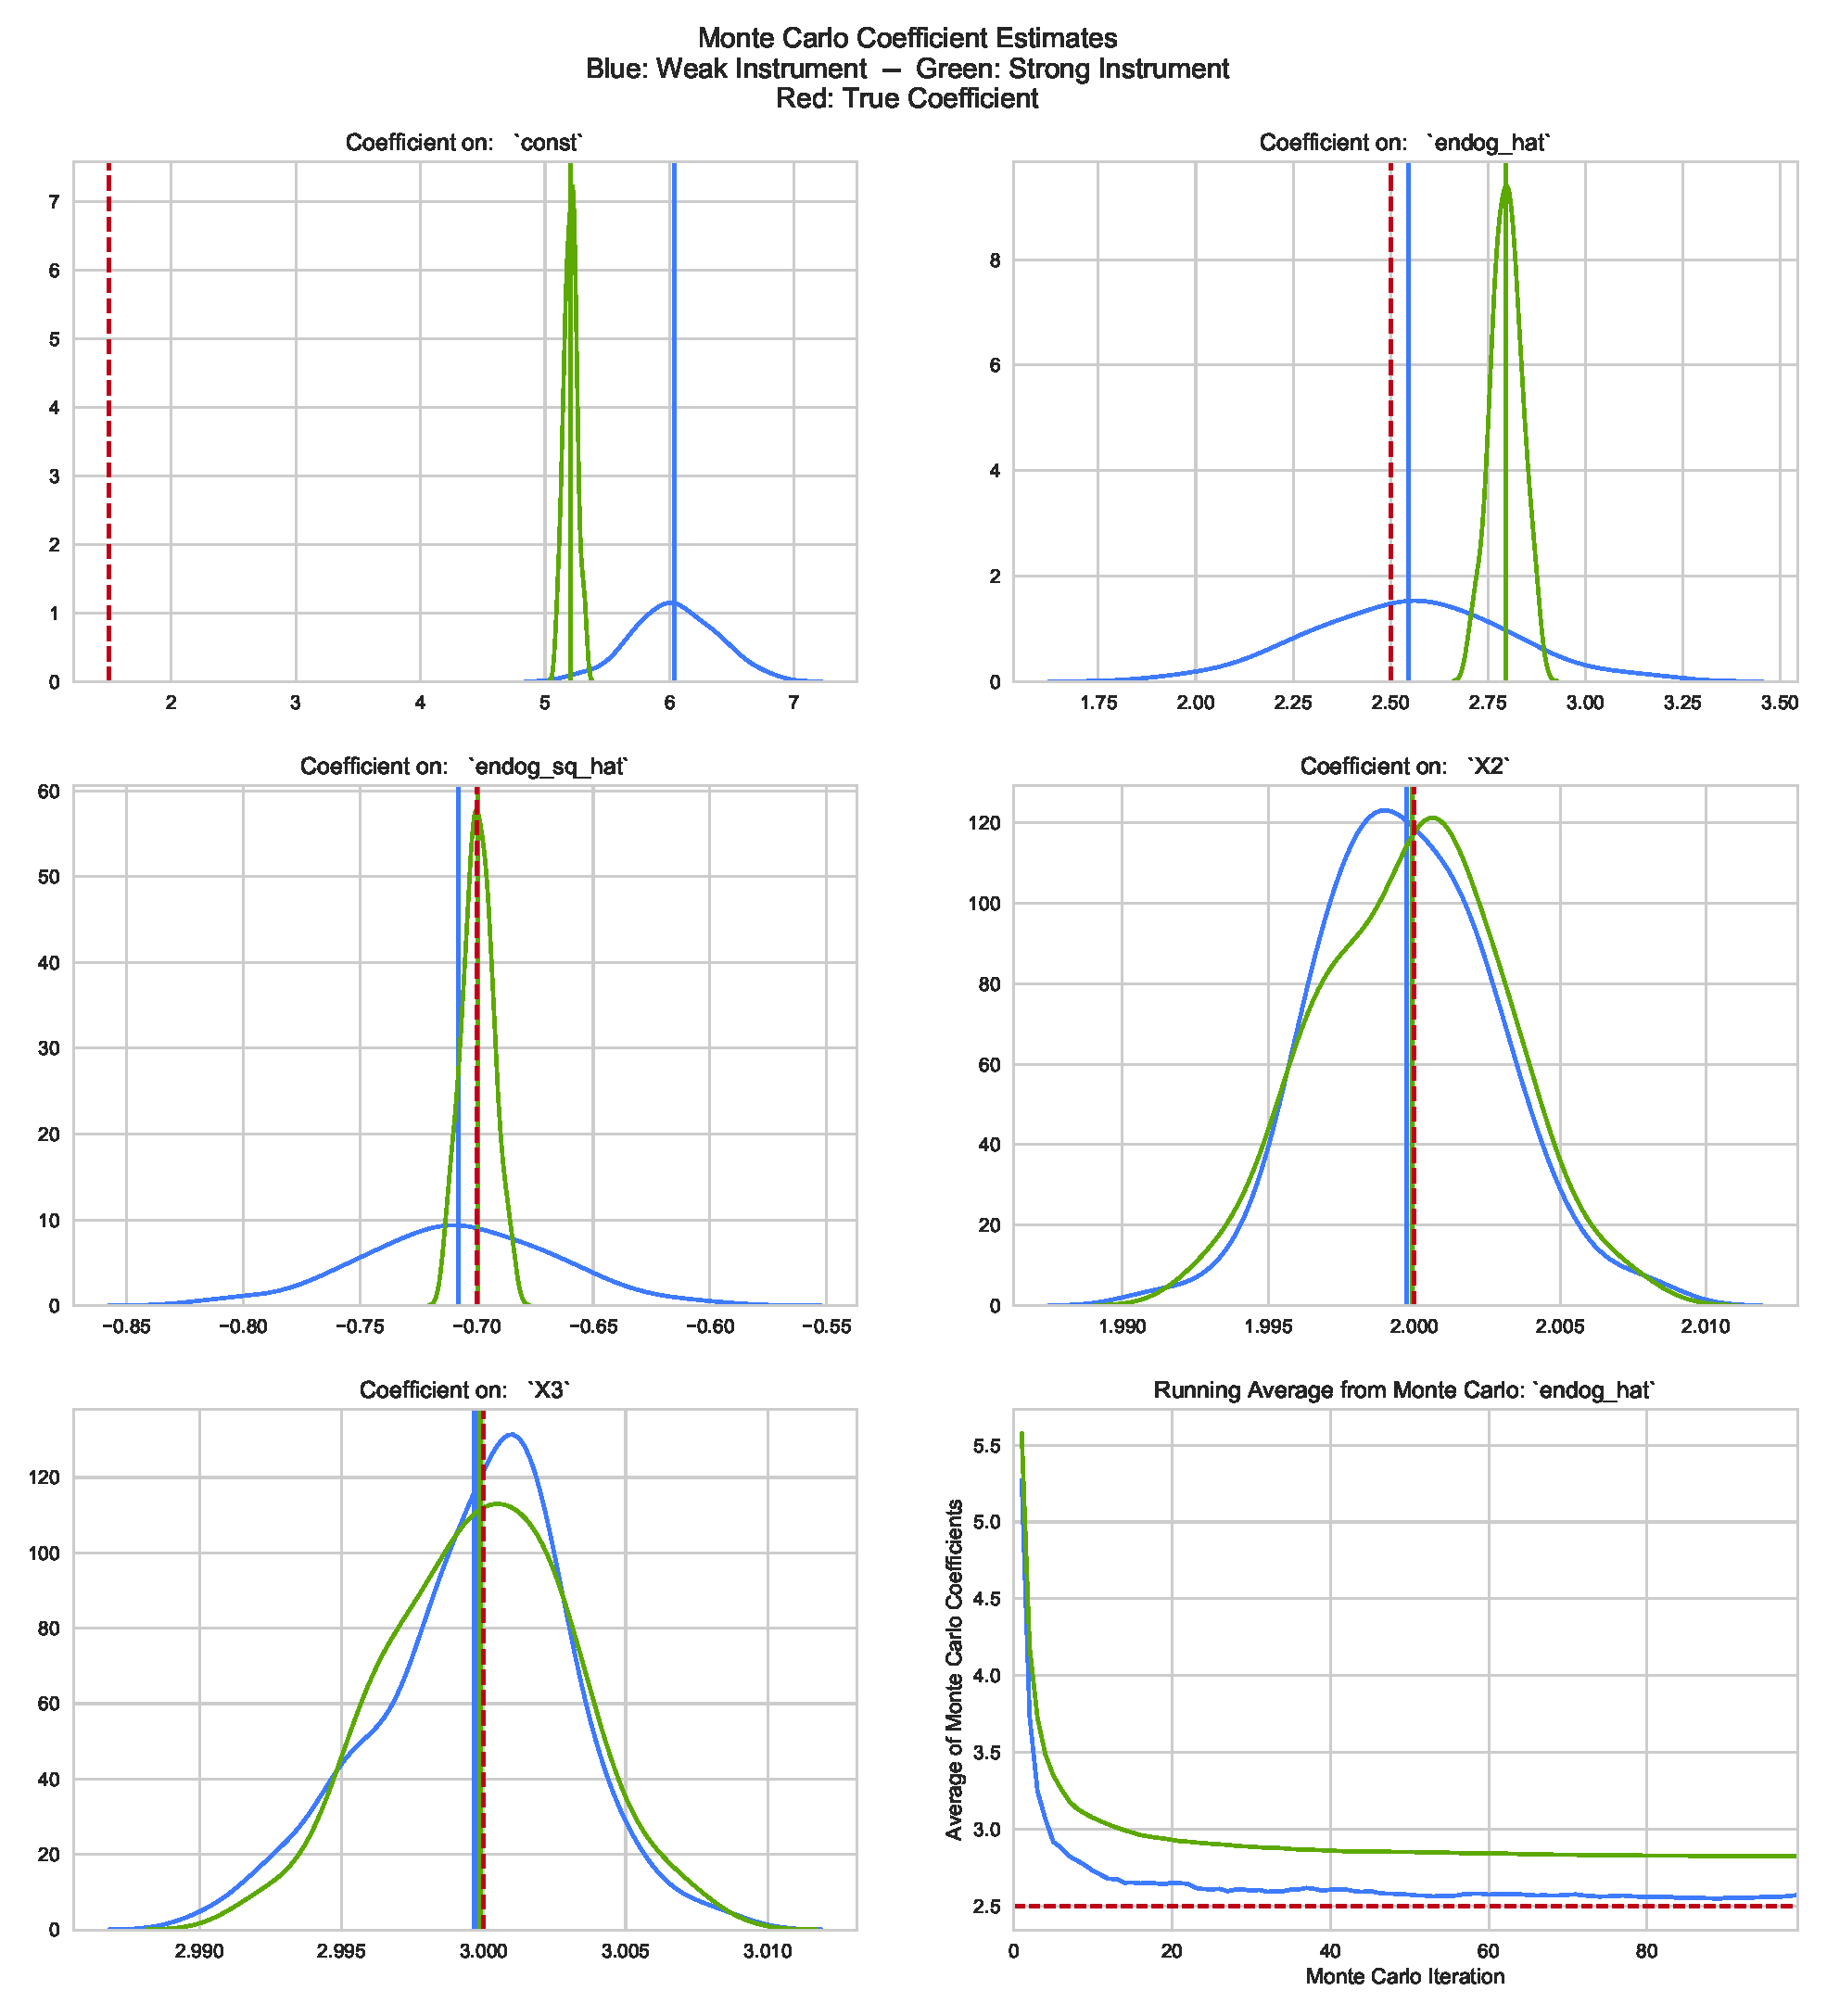
\includegraphics[width=1\linewidth]{figures/MC_strong_and_weak.eps}
\caption{Monte Carlo simulation coefficient estimate distributions}
\label{fig:MC_dists}
\end{figure}

We see that the distribution of the estimated coefficients on the exogenous variables X2 and X3 are unbiased and consistent for both strong and weak instruments (as expected). It also looks as though the estimate on `endog\_sq\_hat` (in section \ref{procedure} we call this ${\wedge \atop x_{i,j}^2}$) is unbiased and consistent, although with weak instruments the variance is much larger\footnote{This is unsurprising - the weaker instruments have more noise introduced into the first stage, which would increase the variance of the coefficient estimates on the instrumented regressors.}. The truly baffling behavior is the estimated coefficient on `endog\_hat` (in section \ref{procedure} we call this $\hat{x}_{i,j}$). With strong instruments we achieve consistency, but severe bias - the true coefficient is not even in the support of the estimated coefficients. And yet with weak instruments it appears we achieve unbiasedness and consistency (albeit a much larger variance again). At first it may seem as though there is a funky collinearity problem between the two generated regressors, but in both the strong and weak instruments the Pearson correlation coefficient is around 0.98 (which leads us to question why there isn't a collinearity problem in the weak instruments approach). While this suggests there is collinearity present, it is unreasonable to think that this collinearity is causing the consistent bias because it is present at equal levels in both the strong and weak instrument settings\footnote{Additionally, if the only issue were multicollinearity then it is unlikely that the bias would be consistent and isolated to only of the instrumented regressors under strong instruments}. Due to time constraints we were unable to find a satisfactory explanation of this behavior, however we plan to continue researching possible sources of the bias under strong instrumentation and will update this document as we make progress.

An additional issue with this nested generated regressor approach is that computing the variance of the coefficient estimates is nontrivial. Due to submission deadlines, there was not enough time to determine whether a consistent estimator for variance of the coefficient estimates exists. We resort to bootstrapping for variance. Currently we use the ``pairs bootstrap", also called ``nonparametric bootstrapping". This involves drawing a sample of the same size (as the original data) from the original data B times, and using the results to estimate the distribution of the estimates. Usually one would report the average bootstrapped estimate as the final estimate (this is standard in prediction settings), but in this causal setting we report the coefficient from running the model on the full sample, and estimate the coefficient variances using the variance from the bootstrapping. These approaches should yield the same result (we would expect that when bootstrapping with regressions the average estimates would approach the full sample estimates as $\mathrm{B} \longrightarrow \infty$). Due to time constraints we have settled on using the bootstrapped variance and the full sample estimates. We then use the standard testing procedure\footnote{Note that by using t-test statistics to test for significance, we implicitly assume that the distribution of $\bm{\beta}$ is approximately multivariate normal. The results from our Monte Carlo simulation suggest that this is not an unreasonable assumption when the data are nice. If we did not assume normality we could use confidence intervals from the bootstrapped distribution to test for significance, unfortunately we did not have time to implement this into the estimation procedure.} to test for significance.

One direction of further development is adding different bootstrapping schemes. We would like to build functionality for a Wild Restricted Efficient Bootstrap approach to coefficient variance estimation. The WRE bootstrap preforms well under endogeneity, especially in the case of weak instruments (\cite{wild_boot}).

%~~~~~~~~~~~~~~~~~~
\subsubsection{Implementation}
\textcolor{Green}{[OUTLINE ONLY]}

\textcolor{BrickRed}{[Discuss chosen instruments and give motivation for why they might be okay to use, give strong disclaimer that even if they are valid, they are probably weak instruments]} Justification for using 'going out' as instrument is stronger if we explain that we have controls for weekly and daily alcohol consumption (which is one thing that could affect grades through going out independently of studying time) so its not insane to claim that going out is exogenous variation in available studying time once the detrimental effects of going out (namely drinking) are controlled for. not a strong argument at all, but at least a little justification. Also include motivation for creating the artificial instrument instead of just using travel time as an instrument; if we just use travel time then there is still an endogeneity problem because people with higher motivation/ability might be choosing schools further away because of their reputation or course options and they might score higher independently to how much they study (because of their higher ability). Point out that in the Monte Carlo simulation, weak instruments resulted in (seemingly) unbiased consistent estimates for the true coeff, but that the variance was massive - which suggests that we should expect a massive variance on our coeff.s because we have weak instruments (and we do find this in practice, which is nice that bootstrapping scheme is correctly getting the big variance).

\textcolor{BrickRed}{[Report results]} Include plots like the naive ols plots, one for 2SLS and one for Q2SLS. Maybe also include fitted values plot with studytime on x axis and predicted grade on y axis. Actually maybe dont include the fitted values plot? because it seems like what we are interested in is the effect of studytime on grades, \textit{all else held equal}, which would just be the coefficients on studytime. The fitted values would be more about predictions than causal effect of studytime.

\textcolor{Red}{Make sure to highlight that these results are not something that I am confident are actually identifying a causal effect, the instruments are too funky and I still am not sure that I fully understand Q2SLS's asymptotic behavior. Mention that this is more meant to be an exploration of a novel analysis using reproducible/responsible research practices.}


%*******************************************************************************************************************
\newpage
\section{Reproducibility}
The importance of reproducible research has been understood for many years. In 1980 Thomas Mayer said ``Neither originality, logical rigor or any other criterion is ranked as `essential' by so many natural scientists as is replicability". Mayer was focusing on replicable research; unfortunately in the social science replicability is often far harder than reproducibility. When it takes five years and tens of thousands of dollars to collect the data for a single study, it is a difficult proposition to attempt to replicate the study from scratch. Additionally, it is unlikely that Mayer could have foreseen the degree to which data wrangling and programming would penetrate into academic research. This reliance on complex data pipelines and analysis with hundreds of dependencies makes replication a beast of a whole new nature. In the current state of empirical research, reproducing the results is half the battle. This opaqueness has led to many published papers that included results that were `p-hacked' or just included mistakes. Ensuring reproducibility would help alleviate many of these issues, and is a big step on the road to replicability.

Reproducibility has become especially important in the current political environment. The National Association for Scholars' recently published a report in which they advocate for use of the Secret Science Reformation Act (renamed the HONEST Act), which would forbid the Environmental Protection Agency from using any research that is not ``substantially reproducible" (\cite{wired}). The NAS report goes even further and suggests that the bill should encompass all federal agencies and courts. Putting aside the various issues with the act\footnote{The act does not define ``substantially reproducible" with any rigor. It is possible that the flexibility of the act could lead to climate change deniers (and others) to call almost any study not substantially reproducible and bar federal agencies from acting on good research.}, if HONEST were to be expanded to other federal agencies, then policy-oriented research in the social sciences would be forced to adapt. Policy makers would need to see ``substantial reproducibility" before allowing a study to influence their policy decisions. Currently, very few empirical papers could be labeled as even somewhat reproducible, and part of the reason why might be that researchers believe implementing reproducible methods into their projects would be too costly in time and resources (\cite{irreproducible}). Hopefully this paper provides a strong argument showing that conducting empirical research using reproducible methods is not only easy, but beneficial. And that were HONEST to be implemented to a wide degree, research need not be impeded\footnote{Ignoring the issue of data confidentiality.}.

%~~~~~~~~~~~~~~~~~~
\subsection{Current Resources}
There are currently some good sources for empirical researchers looking to set up an organized and scalable workflow. One of the best of these is provided by the Gentzkow \& Shapiro lab (\href{https://github.com/gslab-econ/ra-manual/wiki/Getting-Started}{\textcolor{cyan}{link}}, \cite{GSlab}), it is meant to be an internal reference source for their research assistants, but also serves as an excellent guide for other researchers looking to ensure good internal programming practices (they also provide a more general guide \href{https://web.stanford.edu/~gentzkow/research/CodeAndData.xhtml#magicparlabel-20}{\textcolor{cyan}{here}}). It covers computing environments, project management, version control (through GitHub), and coding principles. These are all indispensable tools from the researcher's point of view as they allow for smooth and standardized workflows that are easily interpreted and can be reused later with ease. The one omission from this guide is reproducible and open sourced research practices. This omission is not surprising because of the lack of a large reproducibility movement within the empirical social sciences. The next sections outline basic suggestions for establishing a workflow that not only ensure good internal practices, but also includes elements that help with reproducibility/replication and open source access.

%~~~~~~~~~~~~~~~~~~
\subsection{Basic Workflow}
One of the most useful tools for empirical researchers is GitHub. GitHub allows for seamless version control and easy collaboration. Version control is extremely useful, allowing researchers to easily view their editing history and past analyses that may have been changed or deleted, this also provides a public ledger documenting the history of the research analysis which can be a useful source for reviewers interested in how a final analysis was settled on\footnote{An additional step that helps reviewers and readers is including annotated analyses (Jupyter Notebooks or Rmarkdown files are excellent for this) that were discarded or not included in the final report. This transparency can help ease suspicion of p-hacking or other unintentional mistakes with analysis or data handling.}. Version control also means that researchers can ``checkout" to a new branch and explore alternative analyses without changing the original files. The collaborative aspect of GitHub allows multiple researchers to work on the same files in tandem and later merge the changes together. GitHub also provides an online hosting service, local repositories can be pushed to their public site with a one line command. This is the most effective way of creating an open access research project, by pushing to a public repository you theoretically allow anybody to clone your repository and run it locally on their own machine. In practice there are certain limitations that can cause problems with running a public repository on different local machine.

One of the most common issues is that the order of analysis is unclear. With large project there are often multiple scripts that clean data, then run different types of analyses, or create figures. If these are run out of order they will just return errors. This is where a Makefile comes in. The original researchers create a Makefile with different so called ``phony" commands, and anybody that downloads the repository can then run these one line commands that are actually doing multiple things in a specific order. In this project we have multiple Makefile commands, for example, \inlinecode{make all} runs all of the python Jupyter Notebooks in the correct order and typesets this pdf from .tex and .bib files and \inlinecode{make clean} deletes all the intermediate data and figures. The Makefile allows someone to clone the repository from GitHub and then simply run on line in terminal \inlinecode{make all} to reproduce the results. Unfortunately this doesn't always work because of the different package versions on different machines, this is where environments come in.

If two machines run different versions of python, or even just different versions of specific packages (like scipy or matplotlib), then the same commands may produce different outputs, which defeats the purpose of the Makefile. Anaconda facilitates creation of custom environments to solve this issue. In this project the environment is specified in the \href{https://github.com/nadavtadelis/Reproducible_Metrics/blob/master/environment.yml}{\textcolor{cyan}{\inlinecode{environment.yml}}} file. It creates a local environment with only the packages that are used in the analysis and their specific versions at the time of the analysis. For example our environment uses python 3.6.4 and pandas 0.22.0. Even if there are updates to pandas in the future that renders the current scripts unusable, they will still produce identical results within this environment. By combining these tools the analysis can be identically reproduced even years after the fact.

For additional information, the notes from Professor Fernando P\'erez's course ``Reproducible and Collaborative Data Science" (Fall 2017) are an excellent resource exploring many useful tools and practices (\href{https://berkeley-stat159-f17.github.io/stat159-f17/}{\textcolor{cyan}{link}}, \cite{stat159}).

%~~~~~~~~~~~~~~~~~~
\subsection{Custom Functions}
Many papers in applied econometrics involve developing custom functions for novel analyses. In some cases the paper is an exploration of this new method of analysis, in which case the researchers usually build a public package with the functions to allow others to use them; a good example of this is \inlinecode{causalTree} package documented \href{https://github.com/susanathey/causalTree}{\textcolor{cyan}{here}} (\cite{causalTree}). However this level of documentation and package creation is not necessarily worth the amount of time it takes when the custom analysis functions are not the main point of the research project. In this case it is still useful to use basic documentation tools and function testing, these steps allow the researcher to go back and easily reuse their previous functions, and makes them more understandable for others who might want to implement them. This is the approach taken in this project. We create multiple custom functions (both for data cleaning and for the unusual Q2SLS procedure) and they can hopefully serve as an example of how to create custom functions that can be used by others without too much hassle. 

One of the easiest steps to take that helps both the researcher and future users is good documentation and commenting. Most programming languages have support for function docstrings\footnote{For example, python supports docstrings formatted as : \inlinecode{'''function docstring'''}.} which should include a description of what the function does, the parameters it takes, the output(s), and possibly an example. This provides a future user with all the necessary information on how to implement the function. Additional inclusion of comments within the function helps explain what specific steps are doing, which is useful for understanding the mechanics and for further development or customization.

Once the researcher has created a nicely formatted function script, the next step is to check that it runs without issues. This is where testing comes in. The most basic method of testing is to simply create a separate script that tests the function in a scenario where the researcher knows exactly what the output should be. This approach is useful for preliminary testing and for testing complicated functions (we use this method for testing the Q2SLS function in the function testing notebook - \href{https://nbviewer.jupyter.org/github/nadavtadelis/Reproducible_Metrics/blob/master/function_testing.ipynb}{\textcolor{cyan}{nbviewer}}, \href{https://github.com/nadavtadelis/Reproducible_Metrics/blob/master/function_testing.ipynb}{\textcolor{cyan}{git}}). Once the function developer has a test case (or cases) that they know the function should always pass, they can incorporate continuous integration (CI). CI usually involves writing a testing script that tests the function and asserts that the output is as expected. A third party service will then check that the function passes the tests every time edits are pushed to the public git repo. We use Travis CI to check our custom functions; the testing script is \href{https://github.com/nadavtadelis/Reproducible_Metrics/blob/master/tests.py}{\textcolor{cyan}{\inlinecode{tests.py}}}, the environment the tests run in is \href{https://github.com/nadavtadelis/Reproducible_Metrics/blob/master/.travis.yml}{\textcolor{cyan}{\inlinecode{.travis.yml}}}, and the build status can be monitored through the badge at the top of the README or on Travis's platform \href{https://travis-ci.org/nadavtadelis/Reproducible_Metrics}{\textcolor{cyan}{here}}. CI is expected in the reproducibility community, and empirical research would greatly benefit from its adoption. It is an easy way of verifying that there are no tricky mistakes being made in any of the analysis steps within a larger research project, as well as continuously checking that all functions pass the predefined tests. These precautions take little time, and provide assurances that no careless errors are being made when implementing in-house developed functions.

%~~~~~~~~~~~~~~~~~~
\subsection{Optional/Additional Elements for Reproducibility}
There are some tools that the open source community has begun using which are useful for empirical reproducibility, but not imperative. Here we cover only two tools from a massive pool of resources. Binder is a tool that allows anyone to view and edit Jupyter Notebooks in an executable environment on a remote server through their browser. This means that even if a reader/reviewer does not want to clone the entire repository to their local machine, they can still run and edit the Jupyter Notebooks used in the analysis by using Binder. Researchers can link to their Binder pages by simply including a badge in their repository's README, or they can link to it \href{https://mybinder.org/v2/gh/nadavtadelis/Reproducible_Metrics/master}{\textcolor{cyan}{directly}}. 

Sphinx is also a useful tool, albeit one that has not been used in this project due to time constraints. Sphinx allows a researcher to render their public git repository as a webpage without too much hassle. While this does not sound all that useful, it is tremendously helpful for readers unfamiliar with git repositories who want to navigate a complicated project with many subdirectories. 

There are many other useful tools that have recently been gaining traction. For example there are many third party apps that will automatically check a repository to see what portion of its functions have CI testing implemented, which can be useful for making sure that all functions are tested in large projects with many researchers. There are new tools like these coming out weekly, and keeping somewhat in the loop can help researchers find which tools work best with their workflow.

We would like to point out that even in research that is meant to stand as an example of a reproducible work, there may be compromises. For example, this project involved creating \LaTeX tables to report the regression results from the analysis in the Jupyter Notebooks. Unfortunately there are no simple ways to port regression results directly from Python\footnote{R has an excellent package, stargazer, which can be used in this fashion.} into a formatted \LaTeX table. Instead we resorted to filling in the tables manually in the .tex file. While this should not be a problem for exact reproduction (none of the values change), it would cause issues if the regression outputs were changed but the .tex file was not edited accordingly. These types of lapses in reproducibility are sometimes difficult to overcome, and in cases such as those it is important to point out any possible issues that they might cause.


%*******************************************************************************************************************
\section{Conclusion}
Maybe include a subsection conclusion in Models after Q2SLS results section, but not here?

\textcolor{BlueGreen}{[Actually, use this section to be a short conclusion of the main points, and refer to potential future work and desirable extensions.]}

%*******************************************************************************************************************
\newpage

\begin{singlespace}
\bibliographystyle{agsm}
\nocite{*} % makes sure that all items in .bib are included in bibliography, even if they aren't cited
\bibliography{tex_stuff/RM_bibliography}
\end{singlespace}

%*******************************************************************************************************************
\newpage
\section{Appendix}

%~~~~~~~~~~~~~~~~~~
\subsection{Data Exploration Figures} \label{appendix_figs}
\textcolor{BrickRed}{[ONLY ONE FIGURE INCLUDED FOR NOW, NEED TO ADD OTHER FIGURES AND SCALE NICELY] - or would this make the doc too long? it would add at least 10 pages, i could just link to the /figures directory}

\begin{figure}[H]
\centering
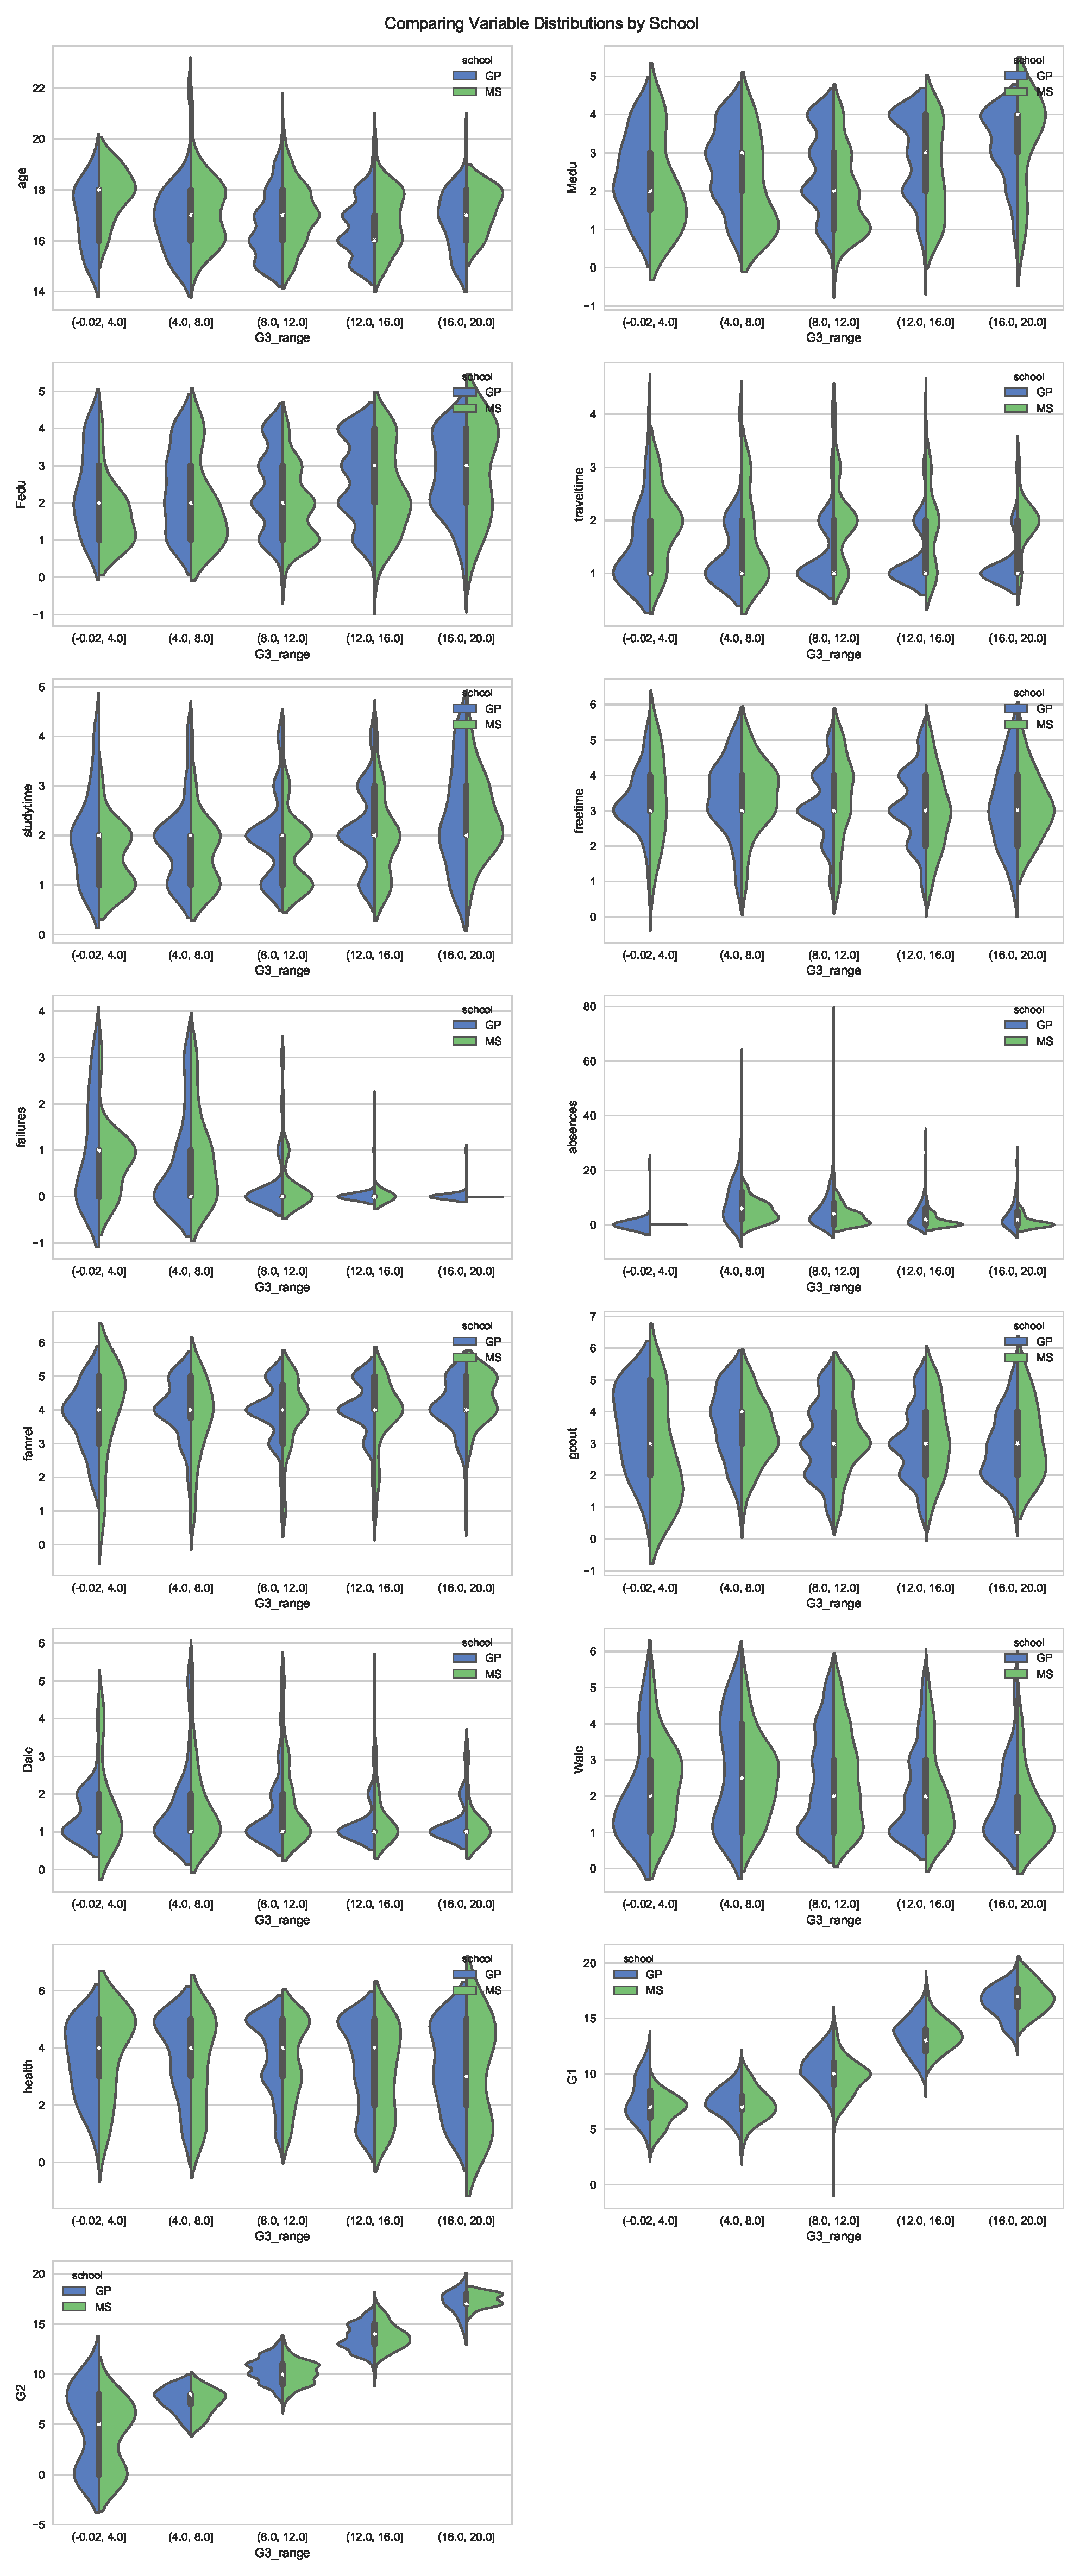
\includegraphics[width=\textwidth,height=0.8\textheight,keepaspectratio]{figures/distrbyschool.eps}
\end{figure}

%\begin{center}
%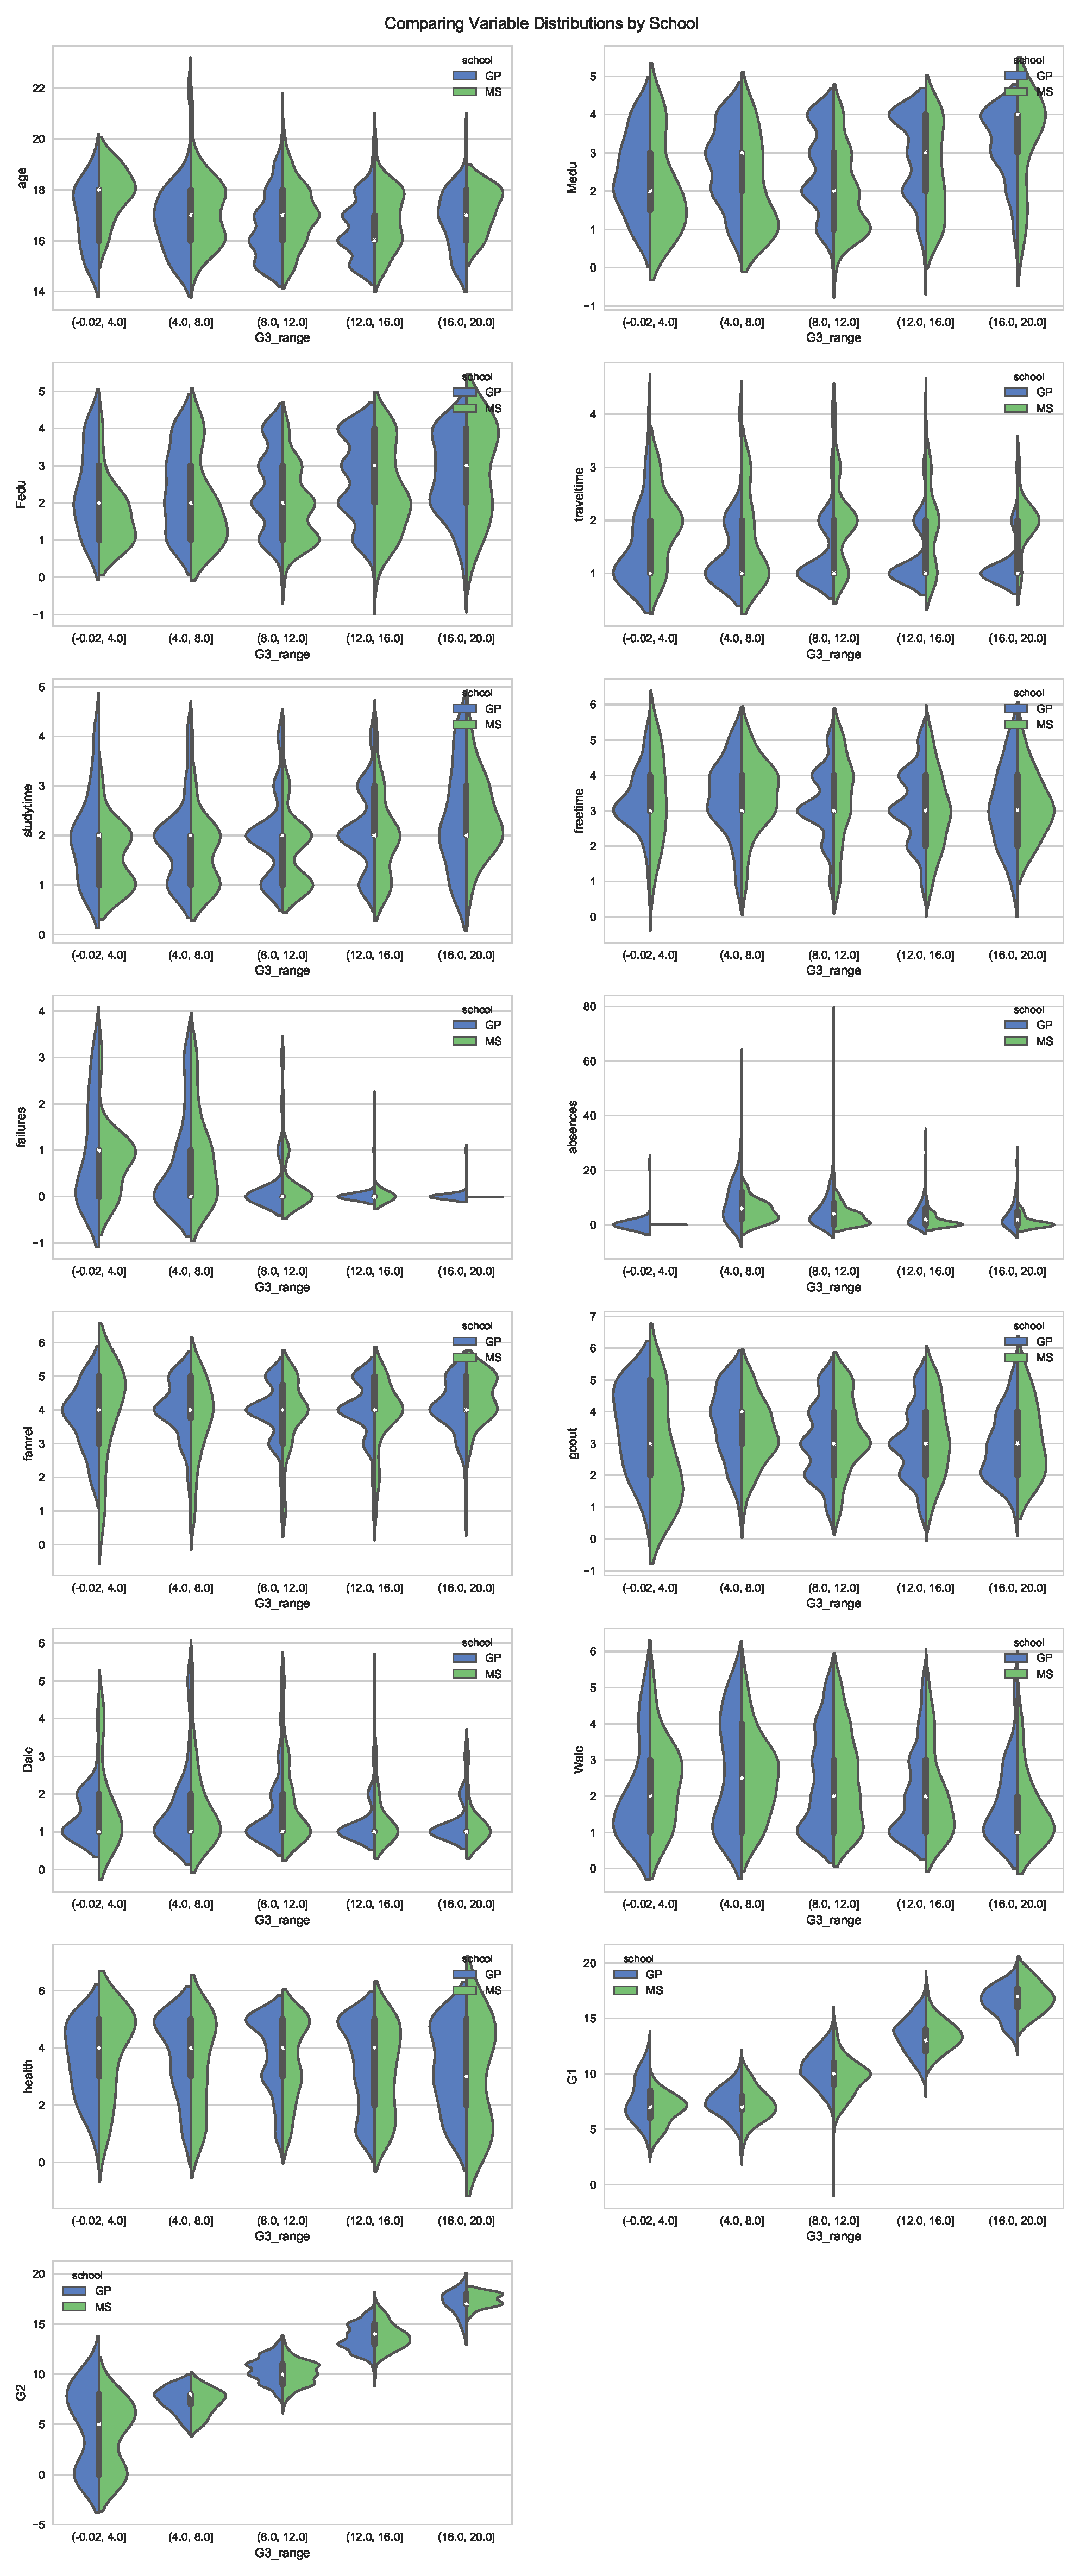
\includegraphics[width=1\linewidth]{figures/distrbyschool.eps}
%\end{center}

%\begin{figure}[h]
%    \centering
%    {{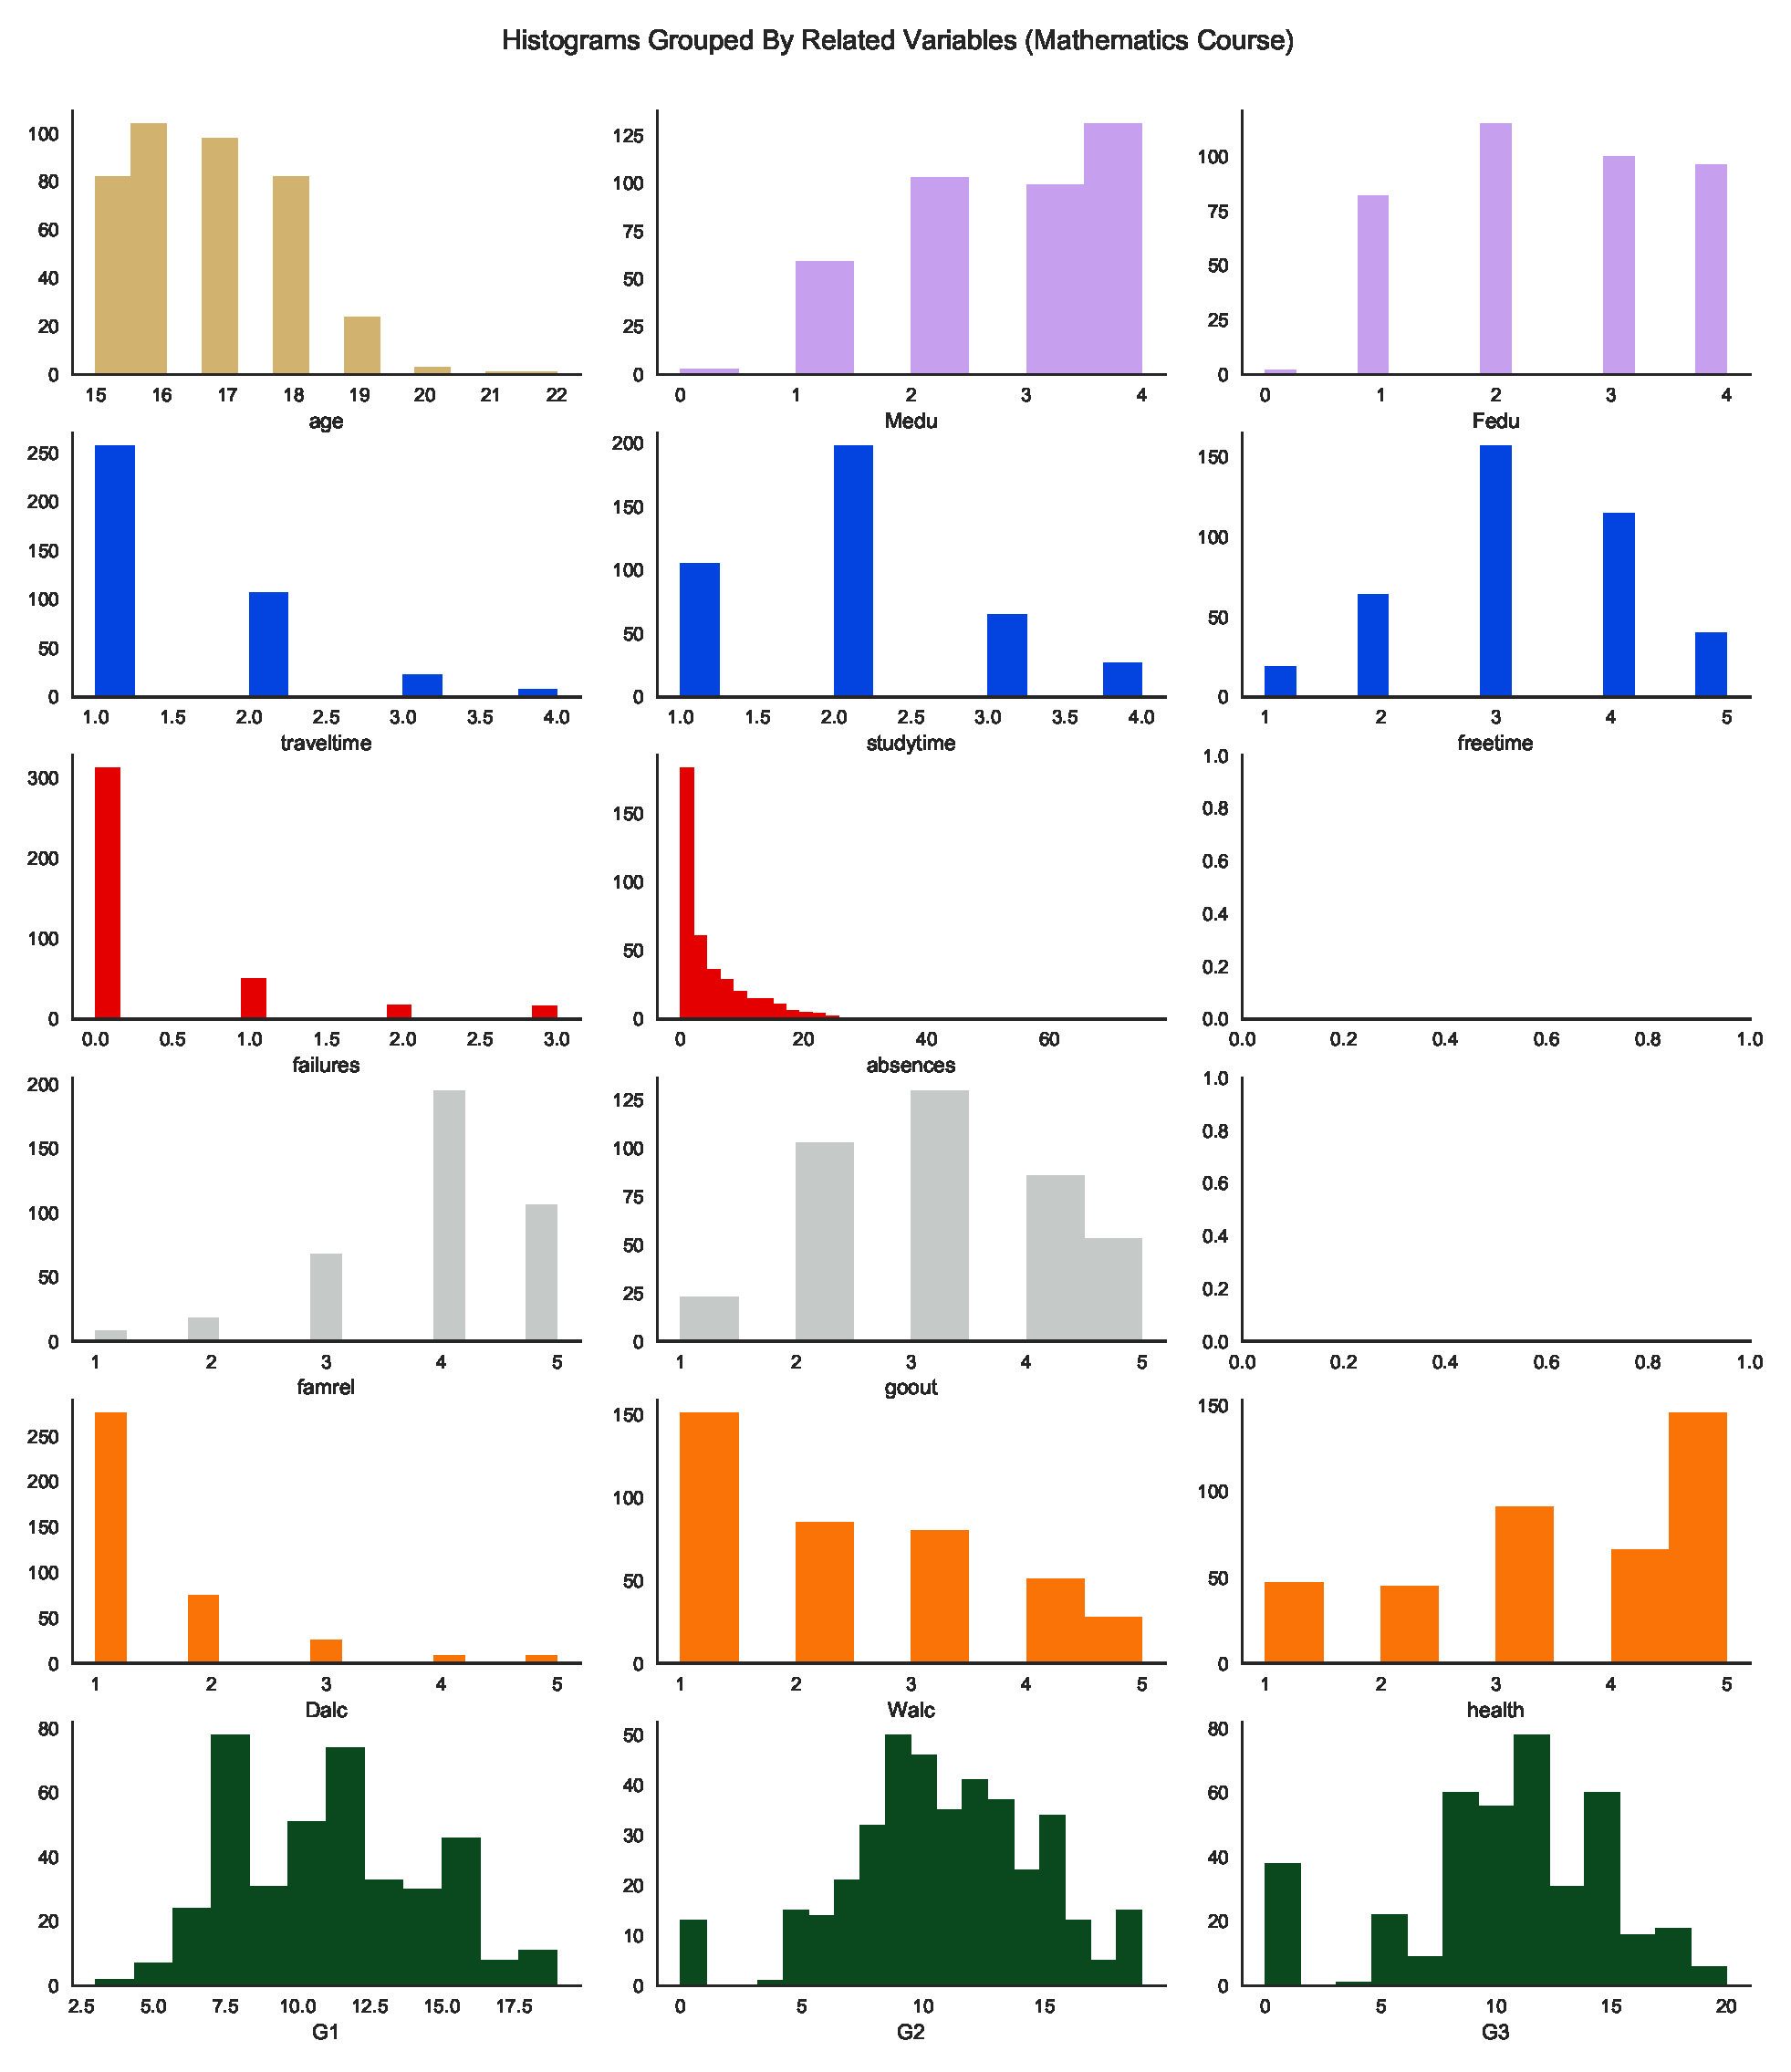
\includegraphics[width=10cm]{figures/quantvar_hist_math.eps} }}
%    \\
%    {{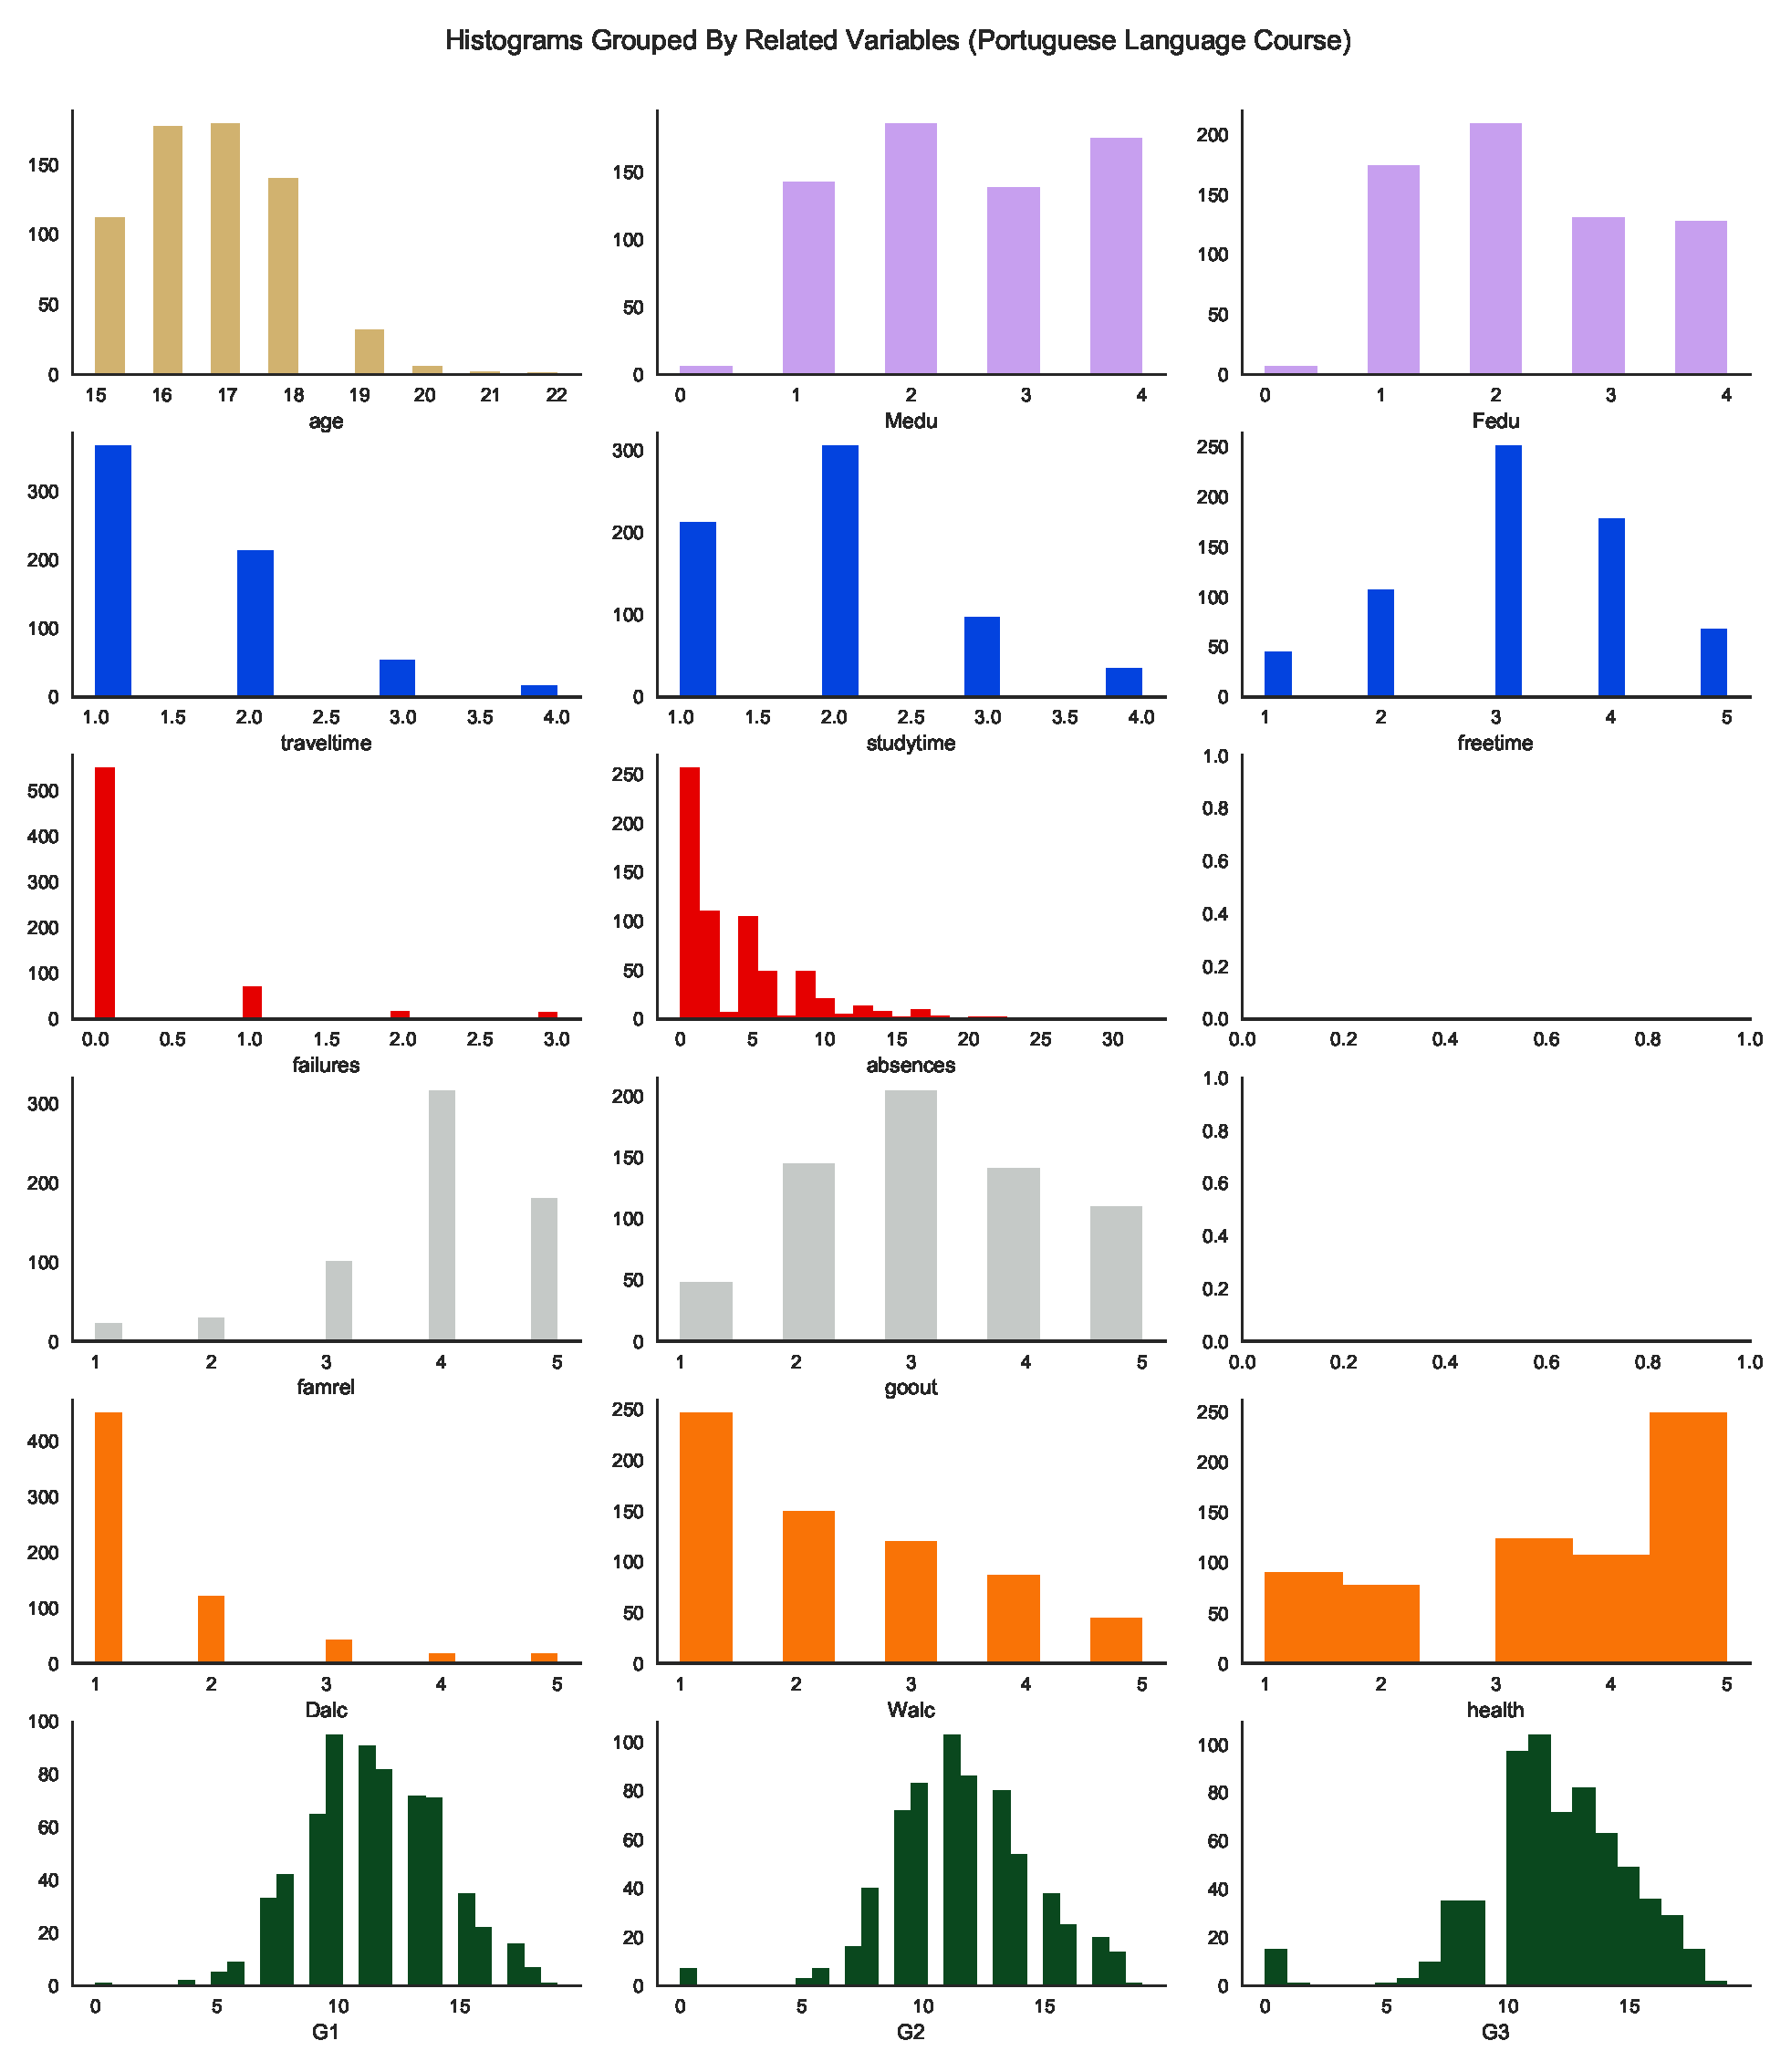
\includegraphics[width=7cm]{figures/quantvar_hist_por.eps} }}
%    \caption{3 Figures arrayed}
%    \label{fig:example}
%\end{figure}

%~~~~~~~~~~~~~~~~~~
\subsection{Naive OLS Extra Models} \label{appendix_naive}

QUESTION: \textcolor{BrickRed}{[Should we report these tables in the main paper and then report tables with all the covariates in the appendix? These would be extra long, and are viewable in the model fitting 1 notebook, so maybe it'd be better to just link to them?]}

%~~~~~~~~~~~~~~~~~~
\subsection{Q2SLS Function Testing Procedure and Monte Carlo} \label{appendix_function_testing}
This section explains in greater detail\footnote{This section re-uses a lot of the comments in the notebook, and for a more complete run through of the Monte Carlo procedure please refer to the notebook.} how the \inlinecode{Quadratic2SLS()} function from \href{https://github.com/nadavtadelis/Reproducible_Metrics/blob/master/quadratic2SLS.py}{\textcolor{cyan}{\inlinecode{quadratic2SLS.py}}} was tested/explored in the function testing notebook - \href{https://nbviewer.jupyter.org/github/nadavtadelis/Reproducible_Metrics/blob/master/function_testing.ipynb}{\textcolor{cyan}{nbviewer}}, \href{https://github.com/nadavtadelis/Reproducible_Metrics/blob/master/function_testing.ipynb}{\textcolor{cyan}{git}}. The notebook serves two purposes, the first goal was to make sure that the function worked as expected with data from a toy data generating process (DGP) simulated through Monte Carlo, and the second was to analyze the asymptotic properties of the estimation procedure in this toy model. The first step was to set up a DGP that was simple, and fit the use case for Q2SLS; i.e. the DGP is quadratic in the endogenous variable.

We first present some motivation for the DGP: we model a toy causal relationship between score on an academic metric $\mathrm{Y}_i$ and various student characteristics. Let $\mathrm{X}_{1, i}$ be student $i$'s weekly hours of studying, then it is reasonable to believe that there are diminishing marginal returns to studying, and that score will be quadratic in studying time. Let $\mathrm{X}_{2, i}$ and $\mathrm{X}_{3, i}$ be some exogenous shifters of score, unrelated to studying time. Let $\mathrm{X}_{4, i}$ be ``ability", an unobserved feature. As $\mathrm{X}_{4, i}$ increases (higher ability), a student will study more, and perhaps their returns to studying will also be greater, hence $\mathrm{X}_{4, i}$ is both correlated with $\mathrm{X}_{1, i}$ and it is used in construction of $\mathrm{Y}_{i}$. Omission of $\mathrm{X}_{4, i}$ in the estimation procedure is where our endogeneity comes from - once it is omitted $\mathrm{X}_{1, i}$ becomes correlated to the error term. The instruments $\mathrm{Z}_{1, i}$ and $\mathrm{Z}_{2, i}$ are some exogenous shifters of studying time unrelated to score $\mathrm{Y}_i$. These instruments are correlated with $\mathrm{X}_{1, i}$ but are not used in constructing $\mathrm{Y}_{i}$. The Monte Carlo simulation pulls from the following DGP:

$$
\begin{aligned}
\begin{pmatrix}
  \mathrm{X}_{1, i}\\
  \mathrm{X}_{2, i}\\
  \mathrm{X}_{3, i}\\
  \mathrm{X}_{4, i}\\
  \mathrm{Z}_{1, i}\\
  \mathrm{Z}_{2, i}
\end{pmatrix} \ &\sim \ N
\begin{bmatrix}
\begin{pmatrix}
  3\\
  -1.5\\
  1.1\\
  2.3\\
  -1\\
  3
\end{pmatrix} \ , \
\begin{pmatrix}
    1 & 0 & 0 & 0.75 & \phi_1 & \phi_2 \\
    0 & 1 & 0 & 0 & 0 & 0 \\
    0 & 0 & 1 & 0 & 0 & 0 \\
    0.75 & 0 & 0 & 1 & 0 & 0 \\
    \phi_1 & 0 & 0 & 0 & 1 & 0 \\
    \phi_2 & 0 & 0 & 0 & 0 & 1 \\
\end{pmatrix}
\end{bmatrix} \\
\varepsilon_i \ &\sim  \ N(0, 1) \\
\mathrm{Y}_i &= 1.5 + 2.5\mathrm{X}_{1, i} - 0.7\mathrm{X}_{1, i}^2 + 2\mathrm{X}_{2, i} + 3\mathrm{X}_{3, i} + 2\mathrm{X}_{4, i} +  \nu_i
\end{aligned}
$$

The estimation procedure is as follows: in each iteration we pull n observations of $[\mathrm{Y}, \mathrm{X}_1, \mathrm{X}_2, \mathrm{X}_3, \mathrm{Z}_1, \mathrm{Z}_2]$. In this case it is clear that omission of $\mathrm{X}_4$ causes $\mathrm{X}_1$ to be endogenous in an estimation of the DGP ($\Cov[\mathrm{X}_{1, i}, \mathrm{X}_{4, i}] \ne 0 \Rightarrow \mathrm{Cov}[\mathrm{X}_{1, i}, \mathrm{\varepsilon}_{i}]  \ne 0 $). We repeat this process 100 times, pulling n = 500,000 observations in each iteration. We run this entire estimation procedure using two DGP's, one with strong\footnote{See section \ref{q2sls_properties} for a note on the strength of instruments in the Q2SLS setting.} instruments ($\phi_1 = 0.8$, $\phi_2 = 0.6$) and one with weak instruments ($\phi_1 = 0.25$, $\phi_2 = 0.2$). Below we plot some of the results from the simulation, for more figures see the notebook or the /figures directory.

\begin{figure}[H]
\centering
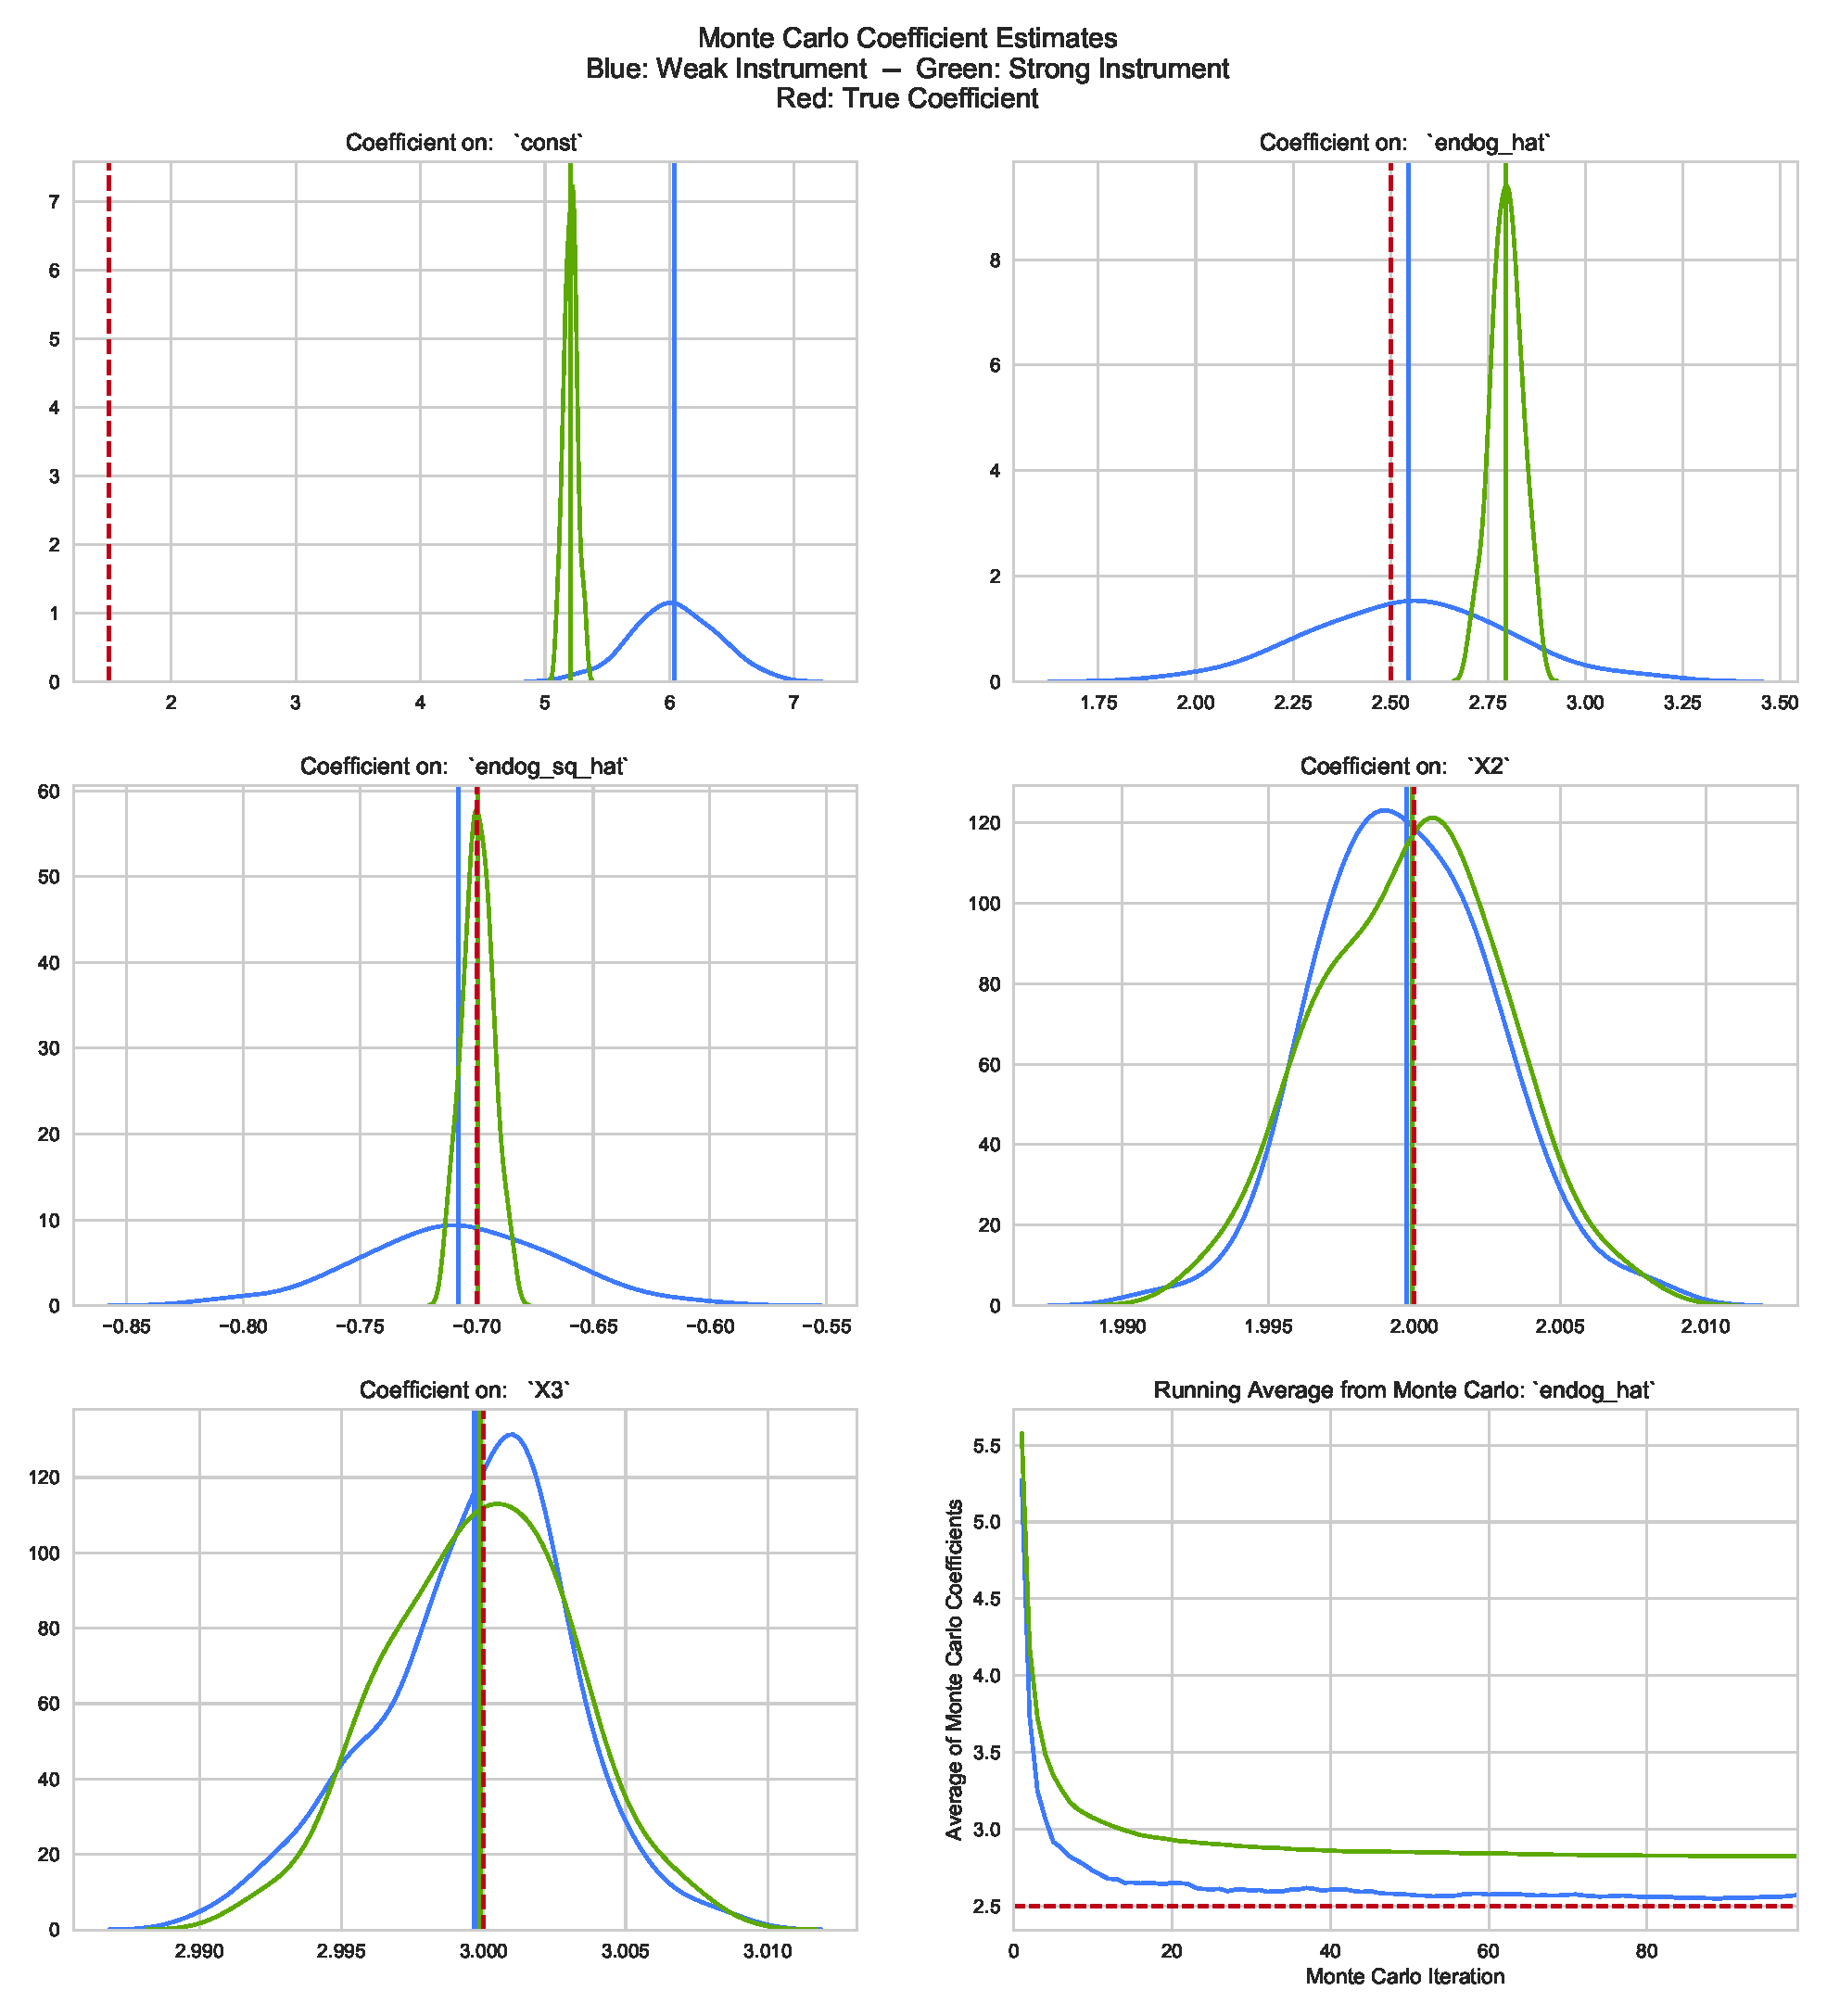
\includegraphics[width=1\linewidth,keepaspectratio]{figures/MC_strong_and_weak.eps}
\caption{This is the same plot from section \ref{q2sls_properties} which shows the distributions of the coefficient estimates}
\end{figure}

\begin{figure}[H]
\centering
\captionsetup{width=0.5\textwidth}
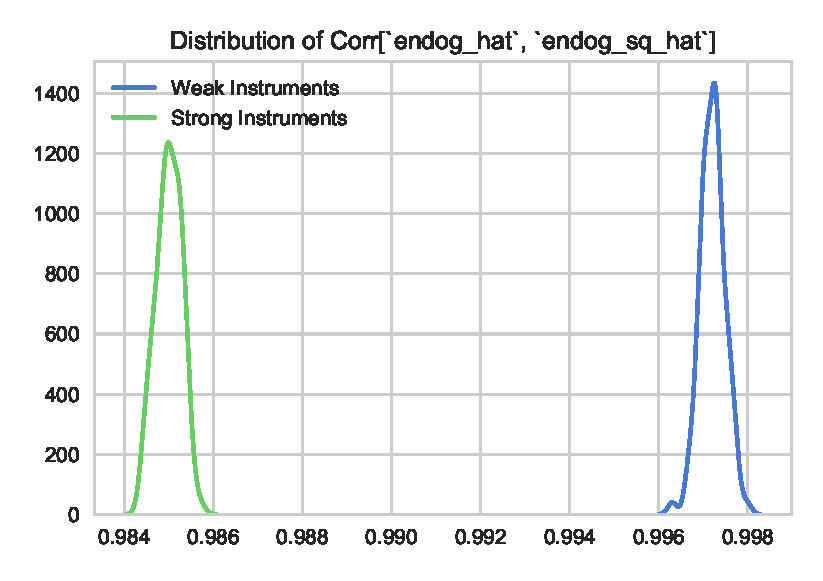
\includegraphics[width=0.5\linewidth,keepaspectratio]{figures/MC_strong_and_weak_corr.eps}
\caption{Correlation between the two generated regressors across the Monte Carlo simulations}
\end{figure}
This figure helped us dismiss the idea that the consistent bias in the strong instruments simulation was caused by multicollinearity. The plot shows that in both strong and weak instrumentation, the generated second stage regressors are collinear, in fact the weaker instrumentation has more collinearity. While this collinearity is not great in and of itself, observing it in both instrumentation settings puts the claim that the bias arises from collinearity into question (otherwise we would expect to see the same bias in both the strong and weak instruments, rather than just the strong).

\begin{figure}[H]
\centering
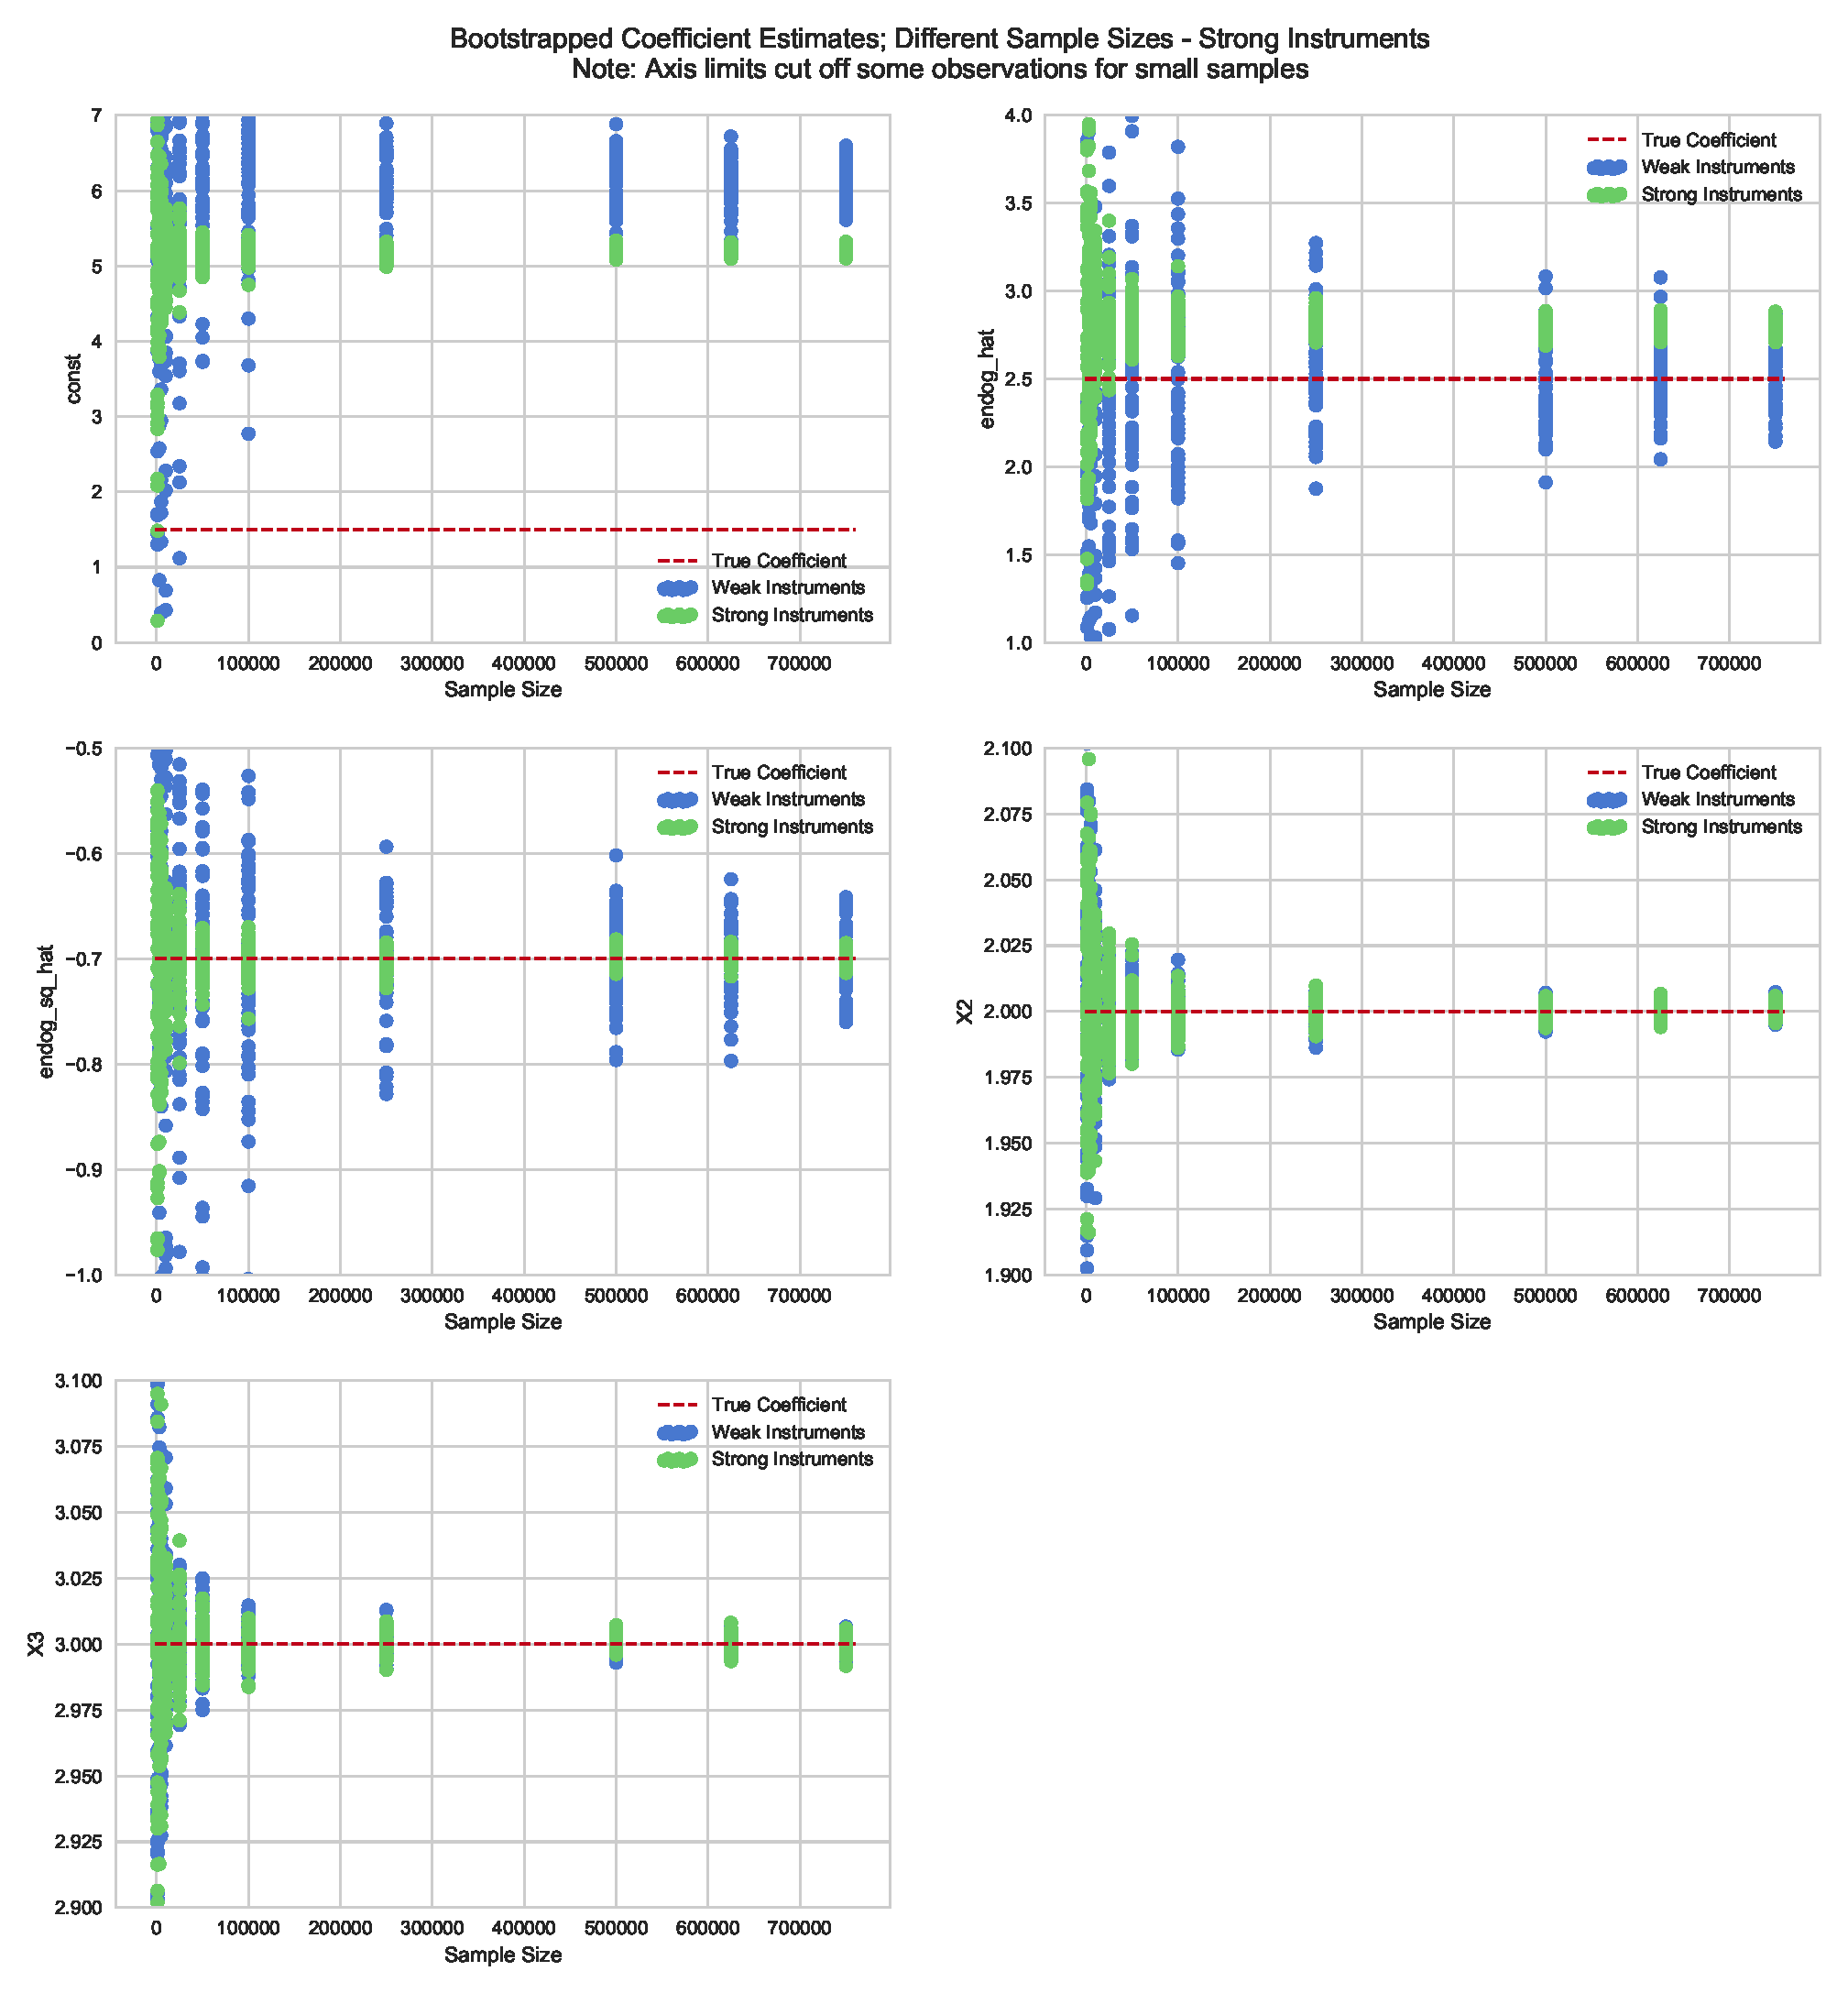
\includegraphics[width=1\linewidth,keepaspectratio]{figures/MC_strong_and_weak_sizes.eps}
\caption{Some support that the estimator is consistent}
\end{figure}

The results from the simulation reassured us that the function was written correctly, but as mentioned previously, the asymptotic behavior was somewhat troubling.


%~~~~~~~~~~~~~~~~~~
\subsection{Q2SLS Extra Models} \label{appendix_q2sls}

\textcolor{BrickRed}{[PUTTING ALL TABLE HERE FOR NOW BECAUSE HAVING TROUBLE PUTTING THEM IN SPECIFIC SECTION]} Note: this Q2SLS table does not have the correct coefficient values, it is just here as a placeholder and to set up the formatting.

\begin{table}[H] \centering
  \caption{Addressing Endogeneity - WRONG VALUES (JUST PLACEHOLDER FOR NOW)}  
\resizebox{\columnwidth}{!}{%
\begin{tabular}{@{\extracolsep{0pt}}lD{.}{.}{-3} D{.}{.}{-3} D{.}{.}{-3}D{.}{.}{-3} D{.}{.}{-3} D{.}{.}{-3} } 
\\[-4ex]\hline 
\hline \\[-1.8ex] 
 & \multicolumn{6}{c}{\textit{Dependent variable:} G3 Grade (Percent)} \\%& \multicolumn{3}{c}{\textit{Dependent variable:} Screening2} \\ 
\cline{2-4} \cline{5-7}
\\[-1.8ex] & \multicolumn{1}{c}{\textit{Both}} & \multicolumn{1}{c}{\textit{Portuguese}} & \multicolumn{1}{c}{\textit{Mathematics}} & \multicolumn{1}{c}{\textit{Both}} & \multicolumn{1}{c}{\textit{Portuguese}} & \multicolumn{1}{c}{\textit{Mathematics}} \\ \ 
\\[-1.8ex] & \multicolumn{1}{c}{(1)} & \multicolumn{1}{c}{(2)} & \multicolumn{1}{c}{(3)} & \multicolumn{1}{c}{(4)} & \multicolumn{1}{c}{(5)} & \multicolumn{1}{c}{(6)} \\ 
\hline \\[-1.8ex] 
  Constant          & 0.4879^{***}  & 0.4686^{***}   & 0.4572^{***}    & 0.4378^{***}    & 0.3049^{***}       & 0.7802^{***}         \\
                          & (0.0161)   & (0.0165)    & (0.0402)     & (0.1103)      & (0.1091)       & (0.2819)         \\[1ex]
  Studytime\_continuous     & 0.0220^{***}  & 0.0268^{***}   & 0.0128       & 0.0155^{***}     & 0.0107^{*}       & 0.0232^{*}          \\
                          & (0.0053)   & (0.0052)    & (0.0113)     & (0.0055)      & (0.0055)       & (0.0126)         \\[1ex]
  Studytime\_continuous\_sq & -0.0010^{***} & -0.0013^{***}  & -0.0005      & -0.0008^{**}     & -0.0004        & -0.0012          \\
                          & (0.0004)   & (0.0004)    & (0.0007)     & (0.0004)      & (0.0003)       & (0.0008)         \\[1ex]
  School\_GP                & 0.0737^{***}  & 0.0856^{***}   & 0.0262       & 0.0371^{**}      & 0.0603^{***}      & -0.0270         \\
                          & (0.0133)   & (0.0142)    & (0.0335)     & (0.0150)      & (0.0160)       & (0.0445)         \\[1ex]
  Course\_math              & -0.0956^{***} &             &              & -0.0959^{***}    &                &                  \\
                          & (0.0128)   &             &              & (0.0150)      &                &                  \\[1ex]
\hline \\[-1.8ex] 
 Model & \textit{2SLS} & \textit{2SLS} & \textit{2SLS} & \textit{Q2SLS} & \textit{Q2SLS} & \textit{Q2SLS} \\[0.2ex]  
\hline \\[-1.8ex] 
Observations & \multicolumn{1}{c}{1,044} & \multicolumn{1}{c}{649} & \multicolumn{1}{c}{395} & \multicolumn{1}{c}{1,044} & \multicolumn{1}{c}{649} & \multicolumn{1}{c}{395} \\
Df & \multicolumn{1}{c}{5} & \multicolumn{1}{c}{4} & \multicolumn{1}{c}{4} & \multicolumn{1}{c}{68} & \multicolumn{1}{c}{67} & \multicolumn{1}{c}{67} \\ 
R$^{2}$ & 0.09       & 0.13        & 0.01         & 0.33          & 0.41           & 0.34             \\ 
Adjusted R$^{2}$ & 0.09       & 0.13        & 0.00         & 0.28          & 0.34           & 0.22             \\ 
F Statistic & 30.11^{***}      & 30.61^{***}       & 1.41         & 7.29^{***}          & 6.03^{***}           & 2.97^{***} \\ 
\hline 
\hline \\[-1.8ex] 
\textit{Note: SE's for Q2SLS are bootstrapped.}  & & & & \multicolumn{3}{r}{$^{*}$p$<$0.1; $^{**}$p$<$0.05; $^{***}$p$<$0.01} \\ 
\end{tabular} 
}
\end{table}


%~~~~~~~~~~~~~~~~~~
\subsection{Miscellanea (?)}


\end{document}




















